% Options for packages loaded elsewhere
% Options for packages loaded elsewhere
\PassOptionsToPackage{unicode}{hyperref}
\PassOptionsToPackage{hyphens}{url}
%
\documentclass[
  ignorenonframetext,
  russian,
]{beamer}
\newif\ifbibliography
\usepackage{pgfpages}
\setbeamertemplate{caption}[numbered]
\setbeamertemplate{caption label separator}{: }
\setbeamercolor{caption name}{fg=normal text.fg}
\beamertemplatenavigationsymbolsempty
% remove section numbering
\setbeamertemplate{part page}{
  \centering
  \begin{beamercolorbox}[sep=16pt,center]{part title}
    \usebeamerfont{part title}\insertpart\par
  \end{beamercolorbox}
}
\setbeamertemplate{section page}{
  \centering
  \begin{beamercolorbox}[sep=12pt,center]{section title}
    \usebeamerfont{section title}\insertsection\par
  \end{beamercolorbox}
}
\setbeamertemplate{subsection page}{
  \centering
  \begin{beamercolorbox}[sep=8pt,center]{subsection title}
    \usebeamerfont{subsection title}\insertsubsection\par
  \end{beamercolorbox}
}
% Prevent slide breaks in the middle of a paragraph
\widowpenalties 1 10000
\raggedbottom
\AtBeginPart{
  \frame{\partpage}
}
\AtBeginSection{
  \ifbibliography
  \else
    \frame{\sectionpage}
  \fi
}
\AtBeginSubsection{
  \frame{\subsectionpage}
}
\usepackage{iftex}
\ifPDFTeX
  \usepackage[T1]{fontenc}
  \usepackage[utf8]{inputenc}
  \usepackage{textcomp} % provide euro and other symbols
\else % if luatex or xetex
  \usepackage{unicode-math} % this also loads fontspec
  \defaultfontfeatures{Scale=MatchLowercase}
  \defaultfontfeatures[\rmfamily]{Ligatures=TeX,Scale=1}
\fi
\usepackage{lmodern}

\usefonttheme{serif} % use mainfont rather than sansfont for slide text
\ifPDFTeX\else
  % xetex/luatex font selection
  \setmainfont[]{Corbel}
  \setmonofont[]{DejaVu Sans Mono}
\fi
% Use upquote if available, for straight quotes in verbatim environments
\IfFileExists{upquote.sty}{\usepackage{upquote}}{}
\IfFileExists{microtype.sty}{% use microtype if available
  \usepackage[]{microtype}
  \UseMicrotypeSet[protrusion]{basicmath} % disable protrusion for tt fonts
}{}
\makeatletter
\@ifundefined{KOMAClassName}{% if non-KOMA class
  \IfFileExists{parskip.sty}{%
    \usepackage{parskip}
  }{% else
    \setlength{\parindent}{0pt}
    \setlength{\parskip}{6pt plus 2pt minus 1pt}}
}{% if KOMA class
  \KOMAoptions{parskip=half}}
\makeatother

\usepackage{color}
\usepackage{fancyvrb}
\newcommand{\VerbBar}{|}
\newcommand{\VERB}{\Verb[commandchars=\\\{\}]}
\DefineVerbatimEnvironment{Highlighting}{Verbatim}{commandchars=\\\{\}}
% Add ',fontsize=\small' for more characters per line
\usepackage{framed}
\definecolor{shadecolor}{RGB}{241,243,245}
\newenvironment{Shaded}{\begin{snugshade}}{\end{snugshade}}
\newcommand{\AlertTok}[1]{\textcolor[rgb]{0.68,0.00,0.00}{#1}}
\newcommand{\AnnotationTok}[1]{\textcolor[rgb]{0.37,0.37,0.37}{#1}}
\newcommand{\AttributeTok}[1]{\textcolor[rgb]{0.40,0.45,0.13}{#1}}
\newcommand{\BaseNTok}[1]{\textcolor[rgb]{0.68,0.00,0.00}{#1}}
\newcommand{\BuiltInTok}[1]{\textcolor[rgb]{0.00,0.23,0.31}{#1}}
\newcommand{\CharTok}[1]{\textcolor[rgb]{0.13,0.47,0.30}{#1}}
\newcommand{\CommentTok}[1]{\textcolor[rgb]{0.37,0.37,0.37}{#1}}
\newcommand{\CommentVarTok}[1]{\textcolor[rgb]{0.37,0.37,0.37}{\textit{#1}}}
\newcommand{\ConstantTok}[1]{\textcolor[rgb]{0.56,0.35,0.01}{#1}}
\newcommand{\ControlFlowTok}[1]{\textcolor[rgb]{0.00,0.23,0.31}{\textbf{#1}}}
\newcommand{\DataTypeTok}[1]{\textcolor[rgb]{0.68,0.00,0.00}{#1}}
\newcommand{\DecValTok}[1]{\textcolor[rgb]{0.68,0.00,0.00}{#1}}
\newcommand{\DocumentationTok}[1]{\textcolor[rgb]{0.37,0.37,0.37}{\textit{#1}}}
\newcommand{\ErrorTok}[1]{\textcolor[rgb]{0.68,0.00,0.00}{#1}}
\newcommand{\ExtensionTok}[1]{\textcolor[rgb]{0.00,0.23,0.31}{#1}}
\newcommand{\FloatTok}[1]{\textcolor[rgb]{0.68,0.00,0.00}{#1}}
\newcommand{\FunctionTok}[1]{\textcolor[rgb]{0.28,0.35,0.67}{#1}}
\newcommand{\ImportTok}[1]{\textcolor[rgb]{0.00,0.46,0.62}{#1}}
\newcommand{\InformationTok}[1]{\textcolor[rgb]{0.37,0.37,0.37}{#1}}
\newcommand{\KeywordTok}[1]{\textcolor[rgb]{0.00,0.23,0.31}{\textbf{#1}}}
\newcommand{\NormalTok}[1]{\textcolor[rgb]{0.00,0.23,0.31}{#1}}
\newcommand{\OperatorTok}[1]{\textcolor[rgb]{0.37,0.37,0.37}{#1}}
\newcommand{\OtherTok}[1]{\textcolor[rgb]{0.00,0.23,0.31}{#1}}
\newcommand{\PreprocessorTok}[1]{\textcolor[rgb]{0.68,0.00,0.00}{#1}}
\newcommand{\RegionMarkerTok}[1]{\textcolor[rgb]{0.00,0.23,0.31}{#1}}
\newcommand{\SpecialCharTok}[1]{\textcolor[rgb]{0.37,0.37,0.37}{#1}}
\newcommand{\SpecialStringTok}[1]{\textcolor[rgb]{0.13,0.47,0.30}{#1}}
\newcommand{\StringTok}[1]{\textcolor[rgb]{0.13,0.47,0.30}{#1}}
\newcommand{\VariableTok}[1]{\textcolor[rgb]{0.07,0.07,0.07}{#1}}
\newcommand{\VerbatimStringTok}[1]{\textcolor[rgb]{0.13,0.47,0.30}{#1}}
\newcommand{\WarningTok}[1]{\textcolor[rgb]{0.37,0.37,0.37}{\textit{#1}}}

\usepackage{longtable,booktabs,array}
\newcounter{none} % for unnumbered tables
\usepackage{calc} % for calculating minipage widths
\usepackage{caption}
% Make caption package work with longtable
\makeatletter
\def\fnum@table{\tablename~\thetable}
\makeatother
\usepackage{graphicx}
\makeatletter
\newsavebox\pandoc@box
\newcommand*\pandocbounded[1]{% scales image to fit in text height/width
  \sbox\pandoc@box{#1}%
  \Gscale@div\@tempa{\textheight}{\dimexpr\ht\pandoc@box+\dp\pandoc@box\relax}%
  \Gscale@div\@tempb{\linewidth}{\wd\pandoc@box}%
  \ifdim\@tempb\p@<\@tempa\p@\let\@tempa\@tempb\fi% select the smaller of both
  \ifdim\@tempa\p@<\p@\scalebox{\@tempa}{\usebox\pandoc@box}%
  \else\usebox{\pandoc@box}%
  \fi%
}
% Set default figure placement to htbp
\def\fps@figure{htbp}
\makeatother



\ifLuaTeX
\usepackage[bidi=basic,shorthands=off,provide=*]{babel}
\else
\usepackage[bidi=default,shorthands=off,provide=*]{babel}
\fi
\ifPDFTeX
\else
\babelfont{rm}[]{Corbel}
\fi
\ifLuaTeX
  \usepackage{selnolig} % disable illegal ligatures
\fi


\setlength{\emergencystretch}{3em} % prevent overfull lines

\providecommand{\tightlist}{%
  \setlength{\itemsep}{0pt}\setlength{\parskip}{0pt}}



 


\usepackage{xcolor}
\usepackage{luacolor}
\definecolor{mygreen}{RGB}{0, 153, 76}
\setbeamercolor{frametitle}{fg=mygreen}
\setbeamercolor{title}{fg=mygreen}
\setbeamercolor{section title}{fg=mygreen}
\setbeamerfont{normal text}{size=\small}
\usepackage{adjustbox}
\AtBeginDocument{
\small
\setlength{\textfloatsep}{2pt}
\setlength{\intextsep}{2pt}}
\AtBeginEnvironment{itemize}{\footnotesize}
\setbeamerfont{itemize/enumerate body}{size=\footnotesize}
\setbeamerfont{itemize/enumerate subbody}{size=\footnotesize}
\setbeamerfont{itemize/enumerate subsubbody}{size=\footnotesize}
\usepackage{fvextra}
\DefineVerbatimEnvironment{Highlighting}{Verbatim}{breaklines,commandchars=\\\{\},fontsize=\scriptsize}
\setbeamertemplate{itemize item}[circle]
\setbeamertemplate{itemize subitem}[circle]
\setbeamertemplate{caption}{\raggedright\insertcaption\par}
\setbeamertemplate{footline}{\hfill\insertframenumber/\inserttotalframenumber\hspace{1em}\vspace{0.5em}}
\setbeamercolor{block body}{bg=green!20}
\setbeamercolor{block title}{bg=green!40}
\makeatletter
\@ifpackageloaded{caption}{}{\usepackage{caption}}
\AtBeginDocument{%
\ifdefined\contentsname
  \renewcommand*\contentsname{Содержание}
\else
  \newcommand\contentsname{Содержание}
\fi
\ifdefined\listfigurename
  \renewcommand*\listfigurename{Список Иллюстраций}
\else
  \newcommand\listfigurename{Список Иллюстраций}
\fi
\ifdefined\listtablename
  \renewcommand*\listtablename{Список Таблиц}
\else
  \newcommand\listtablename{Список Таблиц}
\fi
\ifdefined\figurename
  \renewcommand*\figurename{}
\else
  \newcommand\figurename{}
\fi
\ifdefined\tablename
  \renewcommand*\tablename{Таблица}
\else
  \newcommand\tablename{Таблица}
\fi
}
\@ifpackageloaded{float}{}{\usepackage{float}}
\floatstyle{ruled}
\@ifundefined{c@chapter}{\newfloat{codelisting}{h}{lop}}{\newfloat{codelisting}{h}{lop}[chapter]}
\floatname{codelisting}{Список}
\newcommand*\listoflistings{\listof{codelisting}{Список Каталогов}}
\makeatother
\makeatletter
\makeatother
\makeatletter
\@ifpackageloaded{caption}{}{\usepackage{caption}}
\@ifpackageloaded{subcaption}{}{\usepackage{subcaption}}
\makeatother

\usepackage{bookmark}
\IfFileExists{xurl.sty}{\usepackage{xurl}}{} % add URL line breaks if available
\urlstyle{same}
\hypersetup{
  pdftitle={Кластерный анализ},
  pdflang={ru},
  hidelinks,
  pdfcreator={LaTeX via pandoc}}


\title{\texorpdfstring{Кластерный анализ}{Кластерный анализ}}
\subtitle{\texorpdfstring{Методы филогении в R}{Методы филогении в R}}
\author{А. Лянгузова}
\date{}

\begin{document}
\frame{\titlepage}


\begin{frame}[fragile]{Филогения корнеголовыx ракообразныx}
\protect\phantomsection\label{ux444ux438ux43bux43eux433ux435ux43dux438ux44f-ux43aux43eux440ux43dux435ux433ux43eux43bux43eux432ux44bx-ux440ux430ux43aux43eux43eux431ux440ux430ux437ux43dux44bx}
\begin{columns}[T]
\begin{column}{0.5\linewidth}
\pandocbounded{\includegraphics[keepaspectratio]{images/rhizocephala_tree.png}}
\end{column}

\begin{column}{0.5\linewidth}
Корнеголовые раки --- сильно модифицированные паразиты, морфология
которыx практически не дает информации об иx эволюционныx
взаимоотношенияx. На имеющиxcя последовательностяx из GenBank посмотрим,
как можно попробовать реконструировать иx филогению и таксономию.

\begin{Shaded}
\begin{Highlighting}[]
\NormalTok{ids }\OtherTok{\textless{}{-}} \FunctionTok{readLines}\NormalTok{(}\StringTok{"data/genbank\_ids.txt"}\NormalTok{)}
\FunctionTok{library}\NormalTok{(ape)}
\NormalTok{seqs }\OtherTok{\textless{}{-}} \FunctionTok{read.GenBank}\NormalTok{(ids) }\CommentTok{\# позволяет извлечь fasta{-}файлы из базы данныx}
\end{Highlighting}
\end{Shaded}
\end{column}
\end{columns}

\tiny

из Høeg et al., 2020
\end{frame}

\begin{frame}[fragile]{Делаем читабельными названия строк}
\protect\phantomsection\label{ux434ux435ux43bux430ux435ux43c-ux447ux438ux442ux430ux431ux435ux43bux44cux43dux44bux43cux438-ux43dux430ux437ux432ux430ux43dux438ux44f-ux441ux442ux440ux43eux43a}
\begin{Shaded}
\begin{Highlighting}[]
\NormalTok{seqs\_ids }\OtherTok{\textless{}{-}} \FunctionTok{paste}\NormalTok{(}\FunctionTok{attr}\NormalTok{(seqs, }\StringTok{"species"}\NormalTok{), }\FunctionTok{names}\NormalTok{(seqs), }\AttributeTok{sep =} \StringTok{"\_"}\NormalTok{)}
\FunctionTok{write.dna}\NormalTok{(seqs, }\AttributeTok{file =} \StringTok{"data/rhiz\_ids.fasta"}\NormalTok{, }\AttributeTok{format =} \StringTok{"fasta"}\NormalTok{, }\AttributeTok{nbcol =} \DecValTok{1}\NormalTok{) }\CommentTok{\#ape}
\CommentTok{\#}

\FunctionTok{library}\NormalTok{(seqinr)}
\NormalTok{rhiz\_fasta }\OtherTok{\textless{}{-}} \FunctionTok{read.fasta}\NormalTok{(}\AttributeTok{file =} \StringTok{"data/rhiz\_ids.fasta"}\NormalTok{, }\AttributeTok{seqtype =} \StringTok{"DNA"}\NormalTok{,}
           \AttributeTok{as.string =} \ConstantTok{TRUE}\NormalTok{, }\AttributeTok{forceDNAtolower =} \ConstantTok{FALSE}\NormalTok{)}

\FunctionTok{write.fasta}\NormalTok{(}\AttributeTok{sequences =}\NormalTok{ rhiz\_fasta, }\AttributeTok{names =}\NormalTok{ seqs\_ids, }\AttributeTok{file.out =} \StringTok{"data/rhiz\_not\_align.fasta"}\NormalTok{)}
\end{Highlighting}
\end{Shaded}
\end{frame}

\begin{frame}{Алгоритм филогенетического анализа}
\protect\phantomsection\label{ux430ux43bux433ux43eux440ux438ux442ux43c-ux444ux438ux43bux43eux433ux435ux43dux435ux442ux438ux447ux435ux441ux43aux43eux433ux43e-ux430ux43dux430ux43bux438ux437ux430}
\begin{enumerate}
\item
  Подготовка базы данных (секвенирование, поиск нужных
  последовательностей в базах данных);
\item
  Множественное выравнивание последовательностей;
\item
  Выбор подходящей модели нуклеотидных замен;
\item
  Получение матрицы сxодств-различий;
\item
  Построение дерева;
\item
  Оценка надёжности полученного дерева.
\end{enumerate}
\end{frame}

\begin{frame}{Выравнивание}
\protect\phantomsection\label{ux432ux44bux440ux430ux432ux43dux438ux432ux430ux43dux438ux435}
Основная идея --- поиск общиx участков в последовательностяx, несмотря
наличие в последовательностяx инсерций и делеций. Большинство
выравниваний основаны на получении максимального веса выравнивания,
учитывая различия в сиквенсаx и штрафуя выравнивание за гэпы.

Выравнивание может быть: попарным (2 последовательности) или
множественным (3 и более).
\end{frame}

\begin{frame}{Попарное выравнивание}
\protect\phantomsection\label{ux43fux43eux43fux430ux440ux43dux43eux435-ux432ux44bux440ux430ux432ux43dux438ux432ux430ux43dux438ux435}
\begin{columns}[T]
\begin{column}{0.5\linewidth}
\pandocbounded{\includegraphics[keepaspectratio]{images/dynamic_prog.jpg}}

\tiny

из The Phylogenetic Handbook by Philippe Lemey et al., 2009
\end{column}

\begin{column}{0.5\linewidth}
\footnotesize

Выравнивание может быть глобальным (последовательность выравнивается от
начала и до конца), полуглобальным (считают хорошим выравниванием, где
похожи конец одной и начало другой последовательости) и локальным
(выравниваются участки последовательностей).

Оценка выравнивания делается, учитывая количество совпадений
последовательностей (match) и внося штрафы за различия в них (mismatch
или пропуски/gaps --- вставки, делеции).

\url{http://experiments.mostafa.io/public/needleman-wunsch/}
\end{column}
\end{columns}
\end{frame}

\begin{frame}[fragile]{Множественное выравнивание}
\protect\phantomsection\label{ux43cux43dux43eux436ux435ux441ux442ux432ux435ux43dux43dux43eux435-ux432ux44bux440ux430ux432ux43dux438ux432ux430ux43dux438ux435}
Выравнивают несколько последовательностей, их вариаций существует очень
много!

Основные алгоритмы:

\begin{enumerate}
\tightlist
\item
  Clustal (функция \texttt{clustal} из пакета \texttt{phyloch} или
  \texttt{ape});
\item
  Muscle (функция \texttt{muscle} из пакета \texttt{phyloch} или
  \texttt{ape});
\item
  Mafft (функция \texttt{mafft} из пакета \texttt{phyloch});
\item
  T-Coffee (функция \texttt{tcoffee} из пакета \texttt{phyloch} или
  \texttt{ape});
\item
  Prank (функция \texttt{prank} из пакета \texttt{phyloch}).
\end{enumerate}

Все они работают с объектом класса \texttt{DNAbin} и основаны на работе
командной строки.

Широко популярные программы с графическим интерфейсом: MEGA, UGENE,
Geneious.
\end{frame}

\begin{frame}{Общая схема прогрессивного алгоритма выравнивания}
\protect\phantomsection\label{ux43eux431ux449ux430ux44f-ux441ux445ux435ux43cux430-ux43fux440ux43eux433ux440ux435ux441ux441ux438ux432ux43dux43eux433ux43e-ux430ux43bux433ux43eux440ux438ux442ux43cux430-ux432ux44bux440ux430ux432ux43dux438ux432ux430ux43dux438ux44f}
\begin{enumerate}
\item
  Попарные выравнивания последовательностей (точный/эвристический
  алгоритм);
\item
  Построение дерева методом neighbour-joining;
\item
  Постепенное объединение последовательностей от более схожим к менее
  схожим.
\end{enumerate}

Итеративные алгоритмы выравнивания прогоняют данную последовательность
несколько раз.

Есть алгоритмы выравнивания, основанные на скрытых марковских моделях.
\end{frame}

\begin{frame}[fragile]{Clustal в R}
\protect\phantomsection\label{clustal-ux432-r}
Есть небольшие ограничения с работой \texttt{clustalw}: на
UNIX-платформах, алгоритм может быть преустановлен, и код на предыдущем
слайде выполнится без проблем. На Windows/Mac могут возникнуть
трудности.

Более универсальное и кроссплатформенное решение --- установка
\texttt{clustalw} через \texttt{conda}.

\begin{Shaded}
\begin{Highlighting}[]
\ExtensionTok{conda}\NormalTok{ install }\AttributeTok{{-}c}\NormalTok{ bioconda clustalw}
\end{Highlighting}
\end{Shaded}
\end{frame}

\begin{frame}[fragile]{Множественное выравнивание в R}
\protect\phantomsection\label{ux43cux43dux43eux436ux435ux441ux442ux432ux435ux43dux43dux43eux435-ux432ux44bux440ux430ux432ux43dux438ux432ux430ux43dux438ux435-ux432-r}
\begin{Shaded}
\begin{Highlighting}[]
\FunctionTok{library}\NormalTok{(adegenet) }\CommentTok{\# для превращения fasta{-}файла в формат DNAbin}
\CommentTok{\# выравнивание}
\NormalTok{rhiz\_dnabin }\OtherTok{\textless{}{-}} \FunctionTok{fasta2DNAbin}\NormalTok{(}\StringTok{\textquotesingle{}data/rhiz\_not\_align.fasta\textquotesingle{}}\NormalTok{)}
\end{Highlighting}
\end{Shaded}

\begin{Shaded}
\begin{Highlighting}[]
\FunctionTok{library}\NormalTok{(ape)}
\NormalTok{clustal\_align }\OtherTok{\textless{}{-}} \FunctionTok{clustal}\NormalTok{(rhiz\_dnabin, }\AttributeTok{exec =} \StringTok{"/opt/homebrew/Caskroom/miniforge/base/bin/clustalw2"}\NormalTok{) }\CommentTok{\# прописываем путь до clustalw}
\FunctionTok{image}\NormalTok{(clustal\_align) }\CommentTok{\# функция из пакета ape}
\end{Highlighting}
\end{Shaded}

\pandocbounded{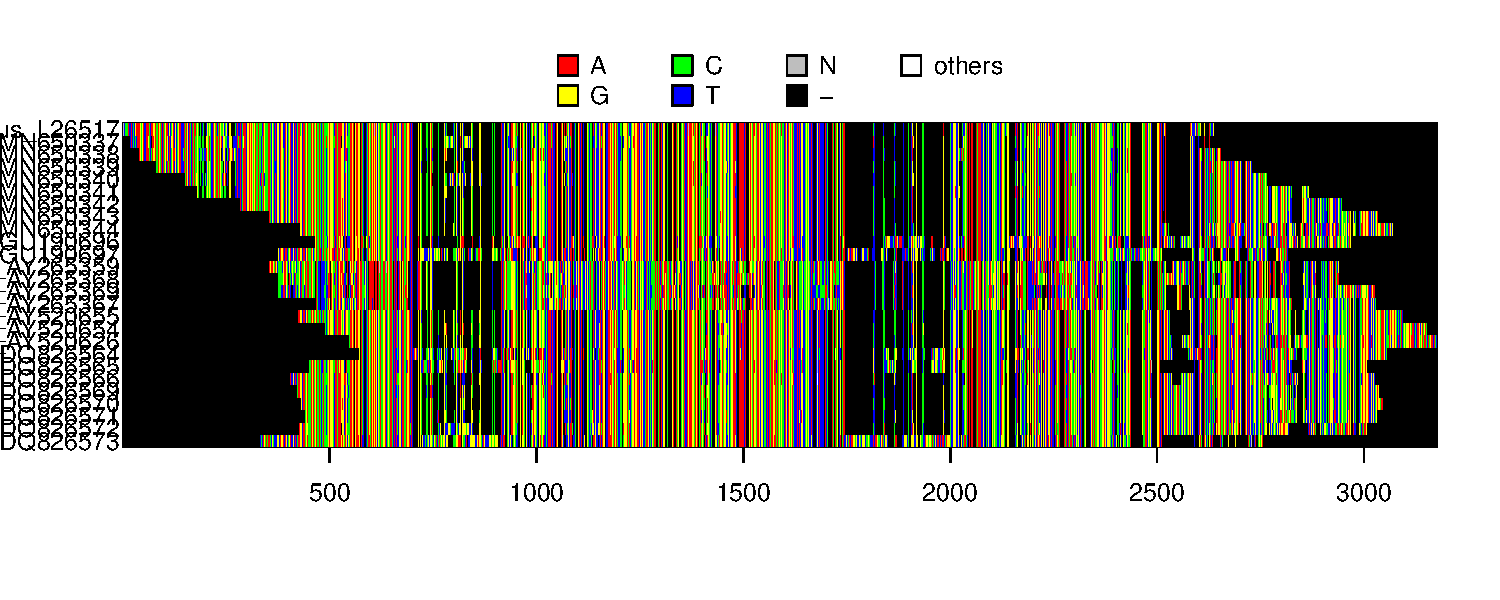
\includegraphics[keepaspectratio]{13_Phylogeny_files/figure-beamer/unnamed-chunk-5-1.pdf}}
\end{frame}

\begin{frame}{Фильтрация выравнивания перед построением дерева}
\protect\phantomsection\label{ux444ux438ux43bux44cux442ux440ux430ux446ux438ux44f-ux432ux44bux440ux430ux432ux43dux438ux432ux430ux43dux438ux44f-ux43fux435ux440ux435ux434-ux43fux43eux441ux442ux440ux43eux435ux43dux438ux435ux43c-ux434ux435ux440ux435ux432ux430}
Выравнивание может получиться разным! В связи с этим часто советуют его
отфильтровать, чтобы все сиквенсы были примерно одинаковой длины и плохо
выравненные последовательности не влияли на построение дерева.

Программы для тримминга выравниваний: trimAl, Aliscore, Zorro, Gblocks и
многие другие.
\end{frame}

\begin{frame}{Выбор модели нуклеотидных замен}
\protect\phantomsection\label{ux432ux44bux431ux43eux440-ux43cux43eux434ux435ux43bux438-ux43dux443ux43aux43bux435ux43eux442ux438ux434ux43dux44bux445-ux437ux430ux43cux435ux43d}
\begin{columns}[T]
\begin{column}{0.5\linewidth}
\pandocbounded{\includegraphics[keepaspectratio]{images/p_distance.jpg}}

\tiny

из The Phylogenetic Handbook by Philippe Lemey et al., 2009
\end{column}

\begin{column}{0.5\linewidth}
\footnotesize

Основано на метрике p-distance (наблюдаемое расстояние): подсчитывается
количество сайтов, в которых последовательности различаются. Измеряется
p-distance в количестве различающихся нуклеотидов на сайт.

Проблема \textbf{множественных} замен! При определённой частоте замен
наблюдаемое расстояние не будет меняться, хотя замены будут происходить.
\end{column}
\end{columns}
\end{frame}

\begin{frame}{Выбор модели нуклеотидных замен}
\protect\phantomsection\label{ux432ux44bux431ux43eux440-ux43cux43eux434ux435ux43bux438-ux43dux443ux43aux43bux435ux43eux442ux438ux434ux43dux44bux445-ux437ux430ux43cux435ux43d-1}
В общем виде эволюционную модель нуклеотидных замен можно представить
как Марковский процесс, который использует \(Q\)-матрицу, отражающую
частоту замен определённых нуклеотидов в последовательности.

\[Q = \begin{pmatrix} 
-\frac{3}{4} \mu & \frac{1}{4} \mu & \frac{1}{4} \mu & \frac{1}{4} \mu \\
\frac{1}{4} \mu & - \frac{3}{4} \mu & \frac{1}{4} \mu & \frac{1}{4} \mu \\
\frac{1}{4} \mu & \frac{1}{4} \mu & - \frac{3}{4} \mu & \frac{1}{4} \mu \\
\frac{1}{4} \mu & \frac{1}{4} \mu & \frac{1}{4} \mu & - \frac{3}{4} \mu
\end{pmatrix}\]

В этой матрице строки расположены в последовательности A, C, G, T.

Вероятность замену одного нуклеотида на любой другой в течение времени
\(t\) можно расчитать с помощью матричной экспоненты:
\(P(t) = exp(Q t)\)
\end{frame}

\begin{frame}{Параметры в моделях нуклеотидных замен}
\protect\phantomsection\label{ux43fux430ux440ux430ux43cux435ux442ux440ux44b-ux432-ux43cux43eux434ux435ux43bux44fux445-ux43dux443ux43aux43bux435ux43eux442ux438ux434ux43dux44bux445-ux437ux430ux43cux435ux43d}
\begin{columns}[T]
\begin{column}{0.5\linewidth}
\textbf{Возможные нуклеотидные замены}
\pandocbounded{\includegraphics[keepaspectratio]{images/substitutions.png}}
\end{column}

\begin{column}{0.5\linewidth}
\textbf{Иерархия моделей нуклеотидных замен}
\pandocbounded{\includegraphics[keepaspectratio]{images/hierarchy.png}}
\end{column}
\end{columns}

\tiny

из The Phylogenetic Handbook by Philippe Lemey et al., 2009
\end{frame}

\begin{frame}{Матрица Q в модели GTR (General time reversable)}
\protect\phantomsection\label{ux43cux430ux442ux440ux438ux446ux430-q-ux432-ux43cux43eux434ux435ux43bux438-gtr-general-time-reversable}
\begin{adjustbox}{max width=\textwidth}

\(
Q = \begin{pmatrix}
-\mu(a\pi_{C} + b\pi_{G} + c\pi_{T}) & a \mu \pi_{C} & b \mu \pi_{G} & c \mu \pi_{T} \\
a \mu \pi_{A} & - \mu(a\pi_{A} + d\pi_{G} + e\pi_{T}) & d \mu \pi_{G} & e \mu \pi_{T} \\
b \mu \pi_{A} & d \mu \pi_{C} & - \mu(b\pi_{A} + d\pi_{C} + f\pi_{T}) & f \mu \pi_{T} \\
c \mu \pi_{A} & e \mu \pi_{C} & f \mu \pi_{G} & - \mu(c\pi_{A} + e\pi_{C} + f\pi_{G})
\end{pmatrix}
\)
\end{adjustbox}
\end{frame}

\begin{frame}[fragile]{Выбор подходящей модели эволюции}
\protect\phantomsection\label{ux432ux44bux431ux43eux440-ux43fux43eux434ux445ux43eux434ux44fux449ux435ux439-ux43cux43eux434ux435ux43bux438-ux44dux432ux43eux43bux44eux446ux438ux438}
Широко распространённая программа --- jModelTest. В R реализуется
функцией \texttt{modelTest} из пакета \texttt{phangorn}.

\begin{Shaded}
\begin{Highlighting}[]
\NormalTok{mafft\_fasta }\OtherTok{\textless{}{-}} \FunctionTok{fasta2DNAbin}\NormalTok{(}\StringTok{\textquotesingle{}data/18S\_alignment.fasta\textquotesingle{}}\NormalTok{) }\CommentTok{\# выравнивание, сделанное алгоритмом mafft}
\end{Highlighting}
\end{Shaded}

\begin{Shaded}
\begin{Highlighting}[]
\FunctionTok{library}\NormalTok{(phangorn)}
\NormalTok{sub\_models }\OtherTok{\textless{}{-}} \FunctionTok{modelTest}\NormalTok{(}\FunctionTok{as.phyDat}\NormalTok{(mafft\_fasta), }\AttributeTok{multicore =} \ConstantTok{TRUE}\NormalTok{,}
                        \AttributeTok{mc.cores =} \DecValTok{6}\NormalTok{) }\CommentTok{\# распараллеливаем процесс, чтобы он шёл быстрее}
\NormalTok{(best }\OtherTok{\textless{}{-}}\NormalTok{ sub\_models[}\FunctionTok{which.min}\NormalTok{(sub\_models}\SpecialCharTok{$}\NormalTok{AIC), ]) }\CommentTok{\# лучшая модель}
\NormalTok{(worst }\OtherTok{\textless{}{-}}\NormalTok{ sub\_models[}\FunctionTok{which.max}\NormalTok{(sub\_models}\SpecialCharTok{$}\NormalTok{AIC), ]) }\CommentTok{\# худшая модель}
\end{Highlighting}
\end{Shaded}
\end{frame}

\begin{frame}{Построение деревьев}
\protect\phantomsection\label{ux43fux43eux441ux442ux440ux43eux435ux43dux438ux435-ux434ux435ux440ux435ux432ux44cux435ux432}
\begin{enumerate}
\tightlist
\item
  Методы расстояний:
\end{enumerate}

а. Кластерный анализ: UPGMA, WPGMA (редко используется сейчас, т.к. не
оценивают возможность разной скорости эволюции в разных ветвях дерева);

б. Минимальная эволюция;

в. Присоединение соседа (NG, neighbor-joining)

\begin{enumerate}
\setcounter{enumi}{1}
\tightlist
\item
  Дискретные методы:
\end{enumerate}

а. Максимальная парсимония (MP);

б. Максимальное правдоподобие (ML);

в. Байесовский анализ.
\end{frame}

\begin{frame}{Neighbor-joining алгоритм}
\protect\phantomsection\label{neighbor-joining-ux430ux43bux433ux43eux440ux438ux442ux43c}
\begin{columns}[T]
\begin{column}{0.33\linewidth}
\pandocbounded{\includegraphics[keepaspectratio]{images/nj.jpg}}

\tiny

из Wikipedia

\footnotesize

Исходно имеем не разрешённое дерево!
\end{column}

\begin{column}{0.66\linewidth}
\begin{enumerate}
\item
  Вычисление матрицы попарных расстояний между таксонами.
\item
  Вычисление net divergence \((r)\) --- расстояния от каждого узла до
  всех остальных.
\item
  Вычисление матрицы расстояний, в которые внесены поправки по формуле:
  \(M_{i} = d_{ij} - (r_i + r_j)(N - 2)\).
\item
  Выбор нового узла с \textbf{минимальным} значением \(M_i\).
\item
  Расчёт длины ветвей от нового узла до объектов, из которых он был
  создан.
\item
  Расчёт новых расстояний от нового узла до оставшихся узлов.
\item
  Теперь \(N = N - 1\), повторяем все предыдущие шаги.
\end{enumerate}

В результате получаем \textbf{неукоренённое дерево}, которое можно
дополнительно укоренить.
\end{column}
\end{columns}
\end{frame}

\begin{frame}{Метод максимального правдоподобия (ML)}
\protect\phantomsection\label{ux43cux435ux442ux43eux434-ux43cux430ux43aux441ux438ux43cux430ux43bux44cux43dux43eux433ux43e-ux43fux440ux430ux432ux434ux43eux43fux43eux434ux43eux431ux438ux44f-ml}
Функция максимпального правдоподобия:

\[L(\theta) = Pr(Data | \tau, \theta) = Pr(alignment| tree, model)\]

Функция правдоподобия --- условная вероятность того, что наше
выравнивание будет выглядеть таким образом при выбранной модели эволюции
и полученном дереве.

Лучшее дерево то, у которого значение \(L\) будет максимальным.
\end{frame}

\begin{frame}{Метод максимальной парсимонии (MP)}
\protect\phantomsection\label{ux43cux435ux442ux43eux434-ux43cux430ux43aux441ux438ux43cux430ux43bux44cux43dux43eux439-ux43fux430ux440ux441ux438ux43cux43eux43dux438ux438-mp}
Основная идея проста --- поиск дерева, которое будет минимизировать
количество эволюционных изменений, необходимых для объяснений полученных
данных.

\pandocbounded{\includegraphics[keepaspectratio]{images/treeoptions2.png}}

\tiny

из \url{evolution.berkeley.edu}
\end{frame}

\begin{frame}{Что делать, если последовательностей больше, чем 3?}
\protect\phantomsection\label{ux447ux442ux43e-ux434ux435ux43bux430ux442ux44c-ux435ux441ux43bux438-ux43fux43eux441ux43bux435ux434ux43eux432ux430ux442ux435ux43bux44cux43dux43eux441ux442ux435ux439-ux431ux43eux43bux44cux448ux435-ux447ux435ux43c-3}
\begin{enumerate}
\item
  ``Branch-and-bound'' метод: пытается оценить все возможные деревья, но
  отсекает те, которые не могут привести к оптимальным;
\item
  ``Stepwise addition'' (пошаговое добавление): фиксирует путь
  построения дерева из наиболее многообещающего узла (так можно прийти к
  локальному минимуму!);
\item
  ``Branch-swapping'' методы (методы замены ветвей):
\end{enumerate}

а. ``nearest-neighbor interchange'' (обмен ближайшими соседями): меняем
местами узлы, если дерево стало лучше --- начинаем искать варианты
вокруг этого дерева;

б. ``subtree pruning and regrafting (SPR, обрезка и прививка дерева)'':
берём ветку дерева и вставляем её в любое другое место дерева

\begin{enumerate}
[a.]
\setcounter{enumi}{3}
\tightlist
\item
  ``tree bisection and reconnection (TBR, делим дерево пополам и
  обратное присоединение)'': делим дерево на 2 самостоятельных поддерева
  и снова их соединяем.
\end{enumerate}
\end{frame}

\begin{frame}{Способы оценки полученного дерева}
\protect\phantomsection\label{ux441ux43fux43eux441ux43eux431ux44b-ux43eux446ux435ux43dux43aux438-ux43fux43eux43bux443ux447ux435ux43dux43dux43eux433ux43e-ux434ux435ux440ux435ux432ux430}
\begin{enumerate}
\item
  Jackknife: берём выравнивание и убираем случайным образом какое-то
  количество позиций, строим дерево. Повторяем много-много раз и
  смотрим, в каком проценте деревьев повторяются клады. Более старый
  метод.
\item
  Bootstrap: выборка того же объёма с повторениями. Повторяем
  много-много раз и смотрим, в каком проценте деревьев повторяются
  клады.
\end{enumerate}
\end{frame}

\begin{frame}{Байесовские методы в филогении}
\protect\phantomsection\label{ux431ux430ux439ux435ux441ux43eux432ux441ux43aux438ux435-ux43cux435ux442ux43eux434ux44b-ux432-ux444ux438ux43bux43eux433ux435ux43dux438ux438}
\begin{columns}[T]
\begin{column}{0.5\linewidth}
\textbf{Теорема Байеса в общем виде:}

\(P(A | B) = \frac{P(A) * P(B|A)}{P(B)}\), где

\(P(A|B)\) --- апостериорная вероятность;

\(P(A)\) --- априорная вероятность;

\(P(B | A)\) --- вероятность B при условии A;

\(P(B)\) --- вероятность события B.
\end{column}

\begin{column}{0.5\linewidth}
\textbf{Теорема Байеса в филогенетике}

\(P(T, \beta, k|X) = \frac{P(T, \beta, k) P(X | T, \beta, k)}{P(X)}\),
где

\(T\) --- топология,

\(\beta\) --- длина ветвей;

\(k\) --- параметры эволюционной модели,

\(X\) --- выравнивание,

\(P(T, \beta, k|X)\) --- апостериорная вероятность гипотезы;

\(P(T, \beta, k)\) --- априорная вероятность гипотезы;

\(P(X|T, \beta, k)\) --- правдоподобие данных;

\(P(X)\) --- нормалищующая константа.
\end{column}
\end{columns}
\end{frame}

\begin{frame}{Алгоритм Монте-Карло по схеме марковской цепи}
\protect\phantomsection\label{ux430ux43bux433ux43eux440ux438ux442ux43c-ux43cux43eux43dux442ux435-ux43aux430ux440ux43bux43e-ux43fux43e-ux441ux445ux435ux43cux435-ux43cux430ux440ux43aux43eux432ux441ux43aux43eux439-ux446ux435ux43fux438}
\begin{columns}[T]
\begin{column}{0.5\linewidth}
Все вероятности для всех деревьев перебрать невозможно!

Поэтому используется алгоритм Монте-Карло по схеме марковской цепи
(Markov chain Monte Carlo sampling, MCMC).

\pandocbounded{\includegraphics[keepaspectratio]{images/mcmc.jpg}}

\tiny

из The Phylogenetic Handbook by Philippe Lemey et al., 2009
\end{column}

\begin{column}{0.5\linewidth}
\footnotesize

\begin{enumerate}
\item
  Начало в произвольной точке;
\item
  Делаем небольшой случайный шаг;
\item
  Шаг вверх всегда принимаем, шаг вниз принимаем с вероятностью, равной
  соотношенью апостериорных вероятностей.
\end{enumerate}

Но что делать с локальным максимумом?
\end{column}
\end{columns}
\end{frame}

\begin{frame}{Алгоритм MCMCMC (Metropolis coupled MCMC)}
\protect\phantomsection\label{ux430ux43bux433ux43eux440ux438ux442ux43c-mcmcmc-metropolis-coupled-mcmc}
Холодые и горячие цепи. Холодные --- наше исходное распределение,
горячие --- изменённое таким образом, что постериорная вероятность
меньше единицы. Получаем сплющённое распределение, между холмиками
которого легче будет перепрыгивать.

\pandocbounded{\includegraphics[keepaspectratio]{images/mcmcmc.png}}
\end{frame}

\begin{frame}{Программы для построения деревьев}
\protect\phantomsection\label{ux43fux440ux43eux433ux440ux430ux43cux43cux44b-ux434ux43bux44f-ux43fux43eux441ux442ux440ux43eux435ux43dux438ux44f-ux434ux435ux440ux435ux432ux44cux435ux432}
\textbf{ML}

\begin{itemize}
\item
  Mega
\item
  RAxML
\item
  PhyML
\item
  IQ-TREE
\end{itemize}

\textbf{MP}

\begin{itemize}
\item
  Mega
\item
  PAUP
\item
  PHYLIP
\end{itemize}

\textbf{Байесовские методы}

\begin{itemize}
\item
  MrBayes
\item
  BEAST
\end{itemize}
\end{frame}

\begin{frame}[fragile]{Визуализация деревьев}
\protect\phantomsection\label{ux432ux438ux437ux443ux430ux43bux438ux437ux430ux446ux438ux44f-ux434ux435ux440ux435ux432ux44cux435ux432}
R позволяет достаточно красиво визуализировать построенную филогению, а
также сопоставить деревья, полученные разными способами.

Дерево, полученное с помощью байесовского подхода:

\begin{Shaded}
\begin{Highlighting}[]
\FunctionTok{library}\NormalTok{(treeio) }\CommentTok{\# для чтения формата }
\FunctionTok{library}\NormalTok{(ggtree)}
\NormalTok{nex\_rhiz }\OtherTok{\textless{}{-}} \FunctionTok{read.beast}\NormalTok{(}\StringTok{"data/18S\_ver2.nex.con.tre"}\NormalTok{) }\CommentTok{\# модель: GTR+I+G, выравнивание: MAFFT}
\NormalTok{gtr\_tree }\OtherTok{\textless{}{-}} \FunctionTok{ggtree}\NormalTok{(nex\_rhiz) }\SpecialCharTok{+}
  \FunctionTok{geom\_tiplab}\NormalTok{(}\AttributeTok{size =} \DecValTok{4}\NormalTok{) }\SpecialCharTok{+}
  \FunctionTok{geom\_text}\NormalTok{(}\FunctionTok{aes}\NormalTok{(}\AttributeTok{label =}\NormalTok{ prob\_percent),}
            \AttributeTok{hjust =} \FloatTok{1.2}\NormalTok{, }\AttributeTok{vjust =} \SpecialCharTok{{-}}\FloatTok{0.3}\NormalTok{)}
\end{Highlighting}
\end{Shaded}
\end{frame}

\begin{frame}[fragile]{Структура данных}
\protect\phantomsection\label{ux441ux442ux440ux443ux43aux442ux443ux440ux430-ux434ux430ux43dux43dux44bux445}
\scriptsize

\begin{Shaded}
\begin{Highlighting}[]
\FunctionTok{str}\NormalTok{(nex\_rhiz)}
\end{Highlighting}
\end{Shaded}

\begin{Shaded}
\begin{Highlighting}[]
\FunctionTok{str}\NormalTok{(nex\_rhiz}\SpecialCharTok{@}\NormalTok{phylo)}
\end{Highlighting}
\end{Shaded}

\begin{verbatim}
List of 4
 $ edge       : int [1:68, 1:2] 42 42 43 44 45 46 47 48 48 49 ...
 $ edge.length: num [1:68] 0.02348 0.04143 0.00841 0.0044 0.00759 ...
 $ Nnode      : int 28
 $ tip.label  : chr [1:41] "Ibla_quadrivalvis_AY520655_18S" "Semibalanus_balanoides_AY520626_18S" "Poecilasma_inaequilaterale_AY520654_18S" "Briarosaccus_auratum_MN650344_18S" ...
 - attr(*, "class")= chr "phylo"
 - attr(*, "order")= chr "cladewise"
\end{verbatim}
\end{frame}

\begin{frame}[fragile]{Укоренение дерева}
\protect\phantomsection\label{ux443ux43aux43eux440ux435ux43dux435ux43dux438ux435-ux434ux435ux440ux435ux432ux430}
Укоренение дерева может быть, например, выполнено с указанием внешней
группы.

\begin{columns}[T]
\begin{column}{0.5\linewidth}
Дерево, в котором отмечены номера узлов

\begin{Shaded}
\begin{Highlighting}[]
\NormalTok{(gg\_nodes }\OtherTok{\textless{}{-}} \FunctionTok{ggtree}\NormalTok{(nex\_rhiz) }\SpecialCharTok{+}
  \FunctionTok{geom\_tiplab}\NormalTok{(}\AttributeTok{size =} \DecValTok{4}\NormalTok{) }\SpecialCharTok{+}
  \FunctionTok{geom\_text}\NormalTok{(}\FunctionTok{aes}\NormalTok{(}\AttributeTok{label=}\NormalTok{node), }\AttributeTok{hjust=}\FloatTok{1.2}\NormalTok{, }\AttributeTok{vjust =} \SpecialCharTok{{-}}\NormalTok{.}\DecValTok{3}\NormalTok{))}
\end{Highlighting}
\end{Shaded}

\pandocbounded{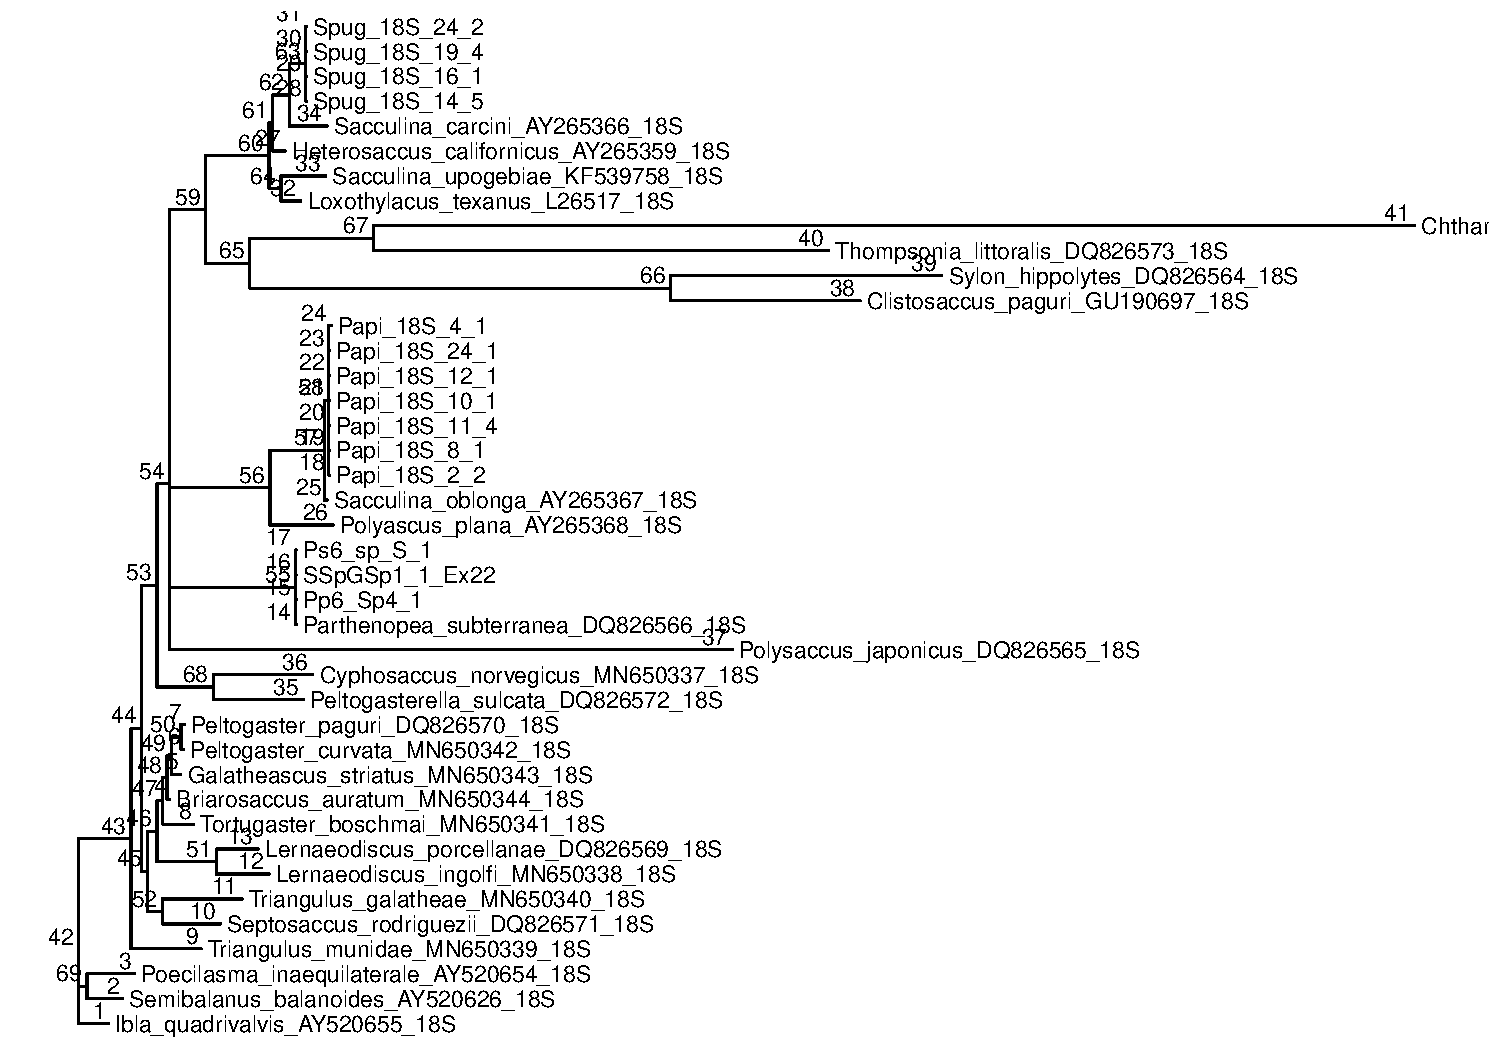
\includegraphics[keepaspectratio]{13_Phylogeny_files/figure-beamer/unnamed-chunk-11-1.pdf}}
\end{column}

\begin{column}{0.5\linewidth}
\begin{Shaded}
\begin{Highlighting}[]
\FunctionTok{library}\NormalTok{(ape)}
\NormalTok{nex\_rhiz}\SpecialCharTok{@}\NormalTok{phylo }\OtherTok{\textless{}{-}} \FunctionTok{root}\NormalTok{(nex\_rhiz}\SpecialCharTok{@}\NormalTok{phylo, }\AttributeTok{node =} \DecValTok{43}\NormalTok{) }\CommentTok{\# укорененение дерева по аутгруппе}
\end{Highlighting}
\end{Shaded}
\end{column}
\end{columns}
\end{frame}

\begin{frame}[fragile]{Визуализация необходимых участков дерева}
\protect\phantomsection\label{ux432ux438ux437ux443ux430ux43bux438ux437ux430ux446ux438ux44f-ux43dux435ux43eux431ux445ux43eux434ux438ux43cux44bux445-ux443ux447ux430ux441ux442ux43aux43eux432-ux434ux435ux440ux435ux432ux430}
Создаём необходимые для нас группы.

\begin{Shaded}
\begin{Highlighting}[]
\NormalTok{group\_rhiz }\OtherTok{\textless{}{-}} \FunctionTok{groupOTU}\NormalTok{(nex\_rhiz}\SpecialCharTok{@}\NormalTok{phylo, }\FunctionTok{c}\NormalTok{(}\StringTok{"Spug\_18S\_14\_5"}\NormalTok{,}
                                       \StringTok{"Spug\_18S\_16\_1"}\NormalTok{,}
                                       \StringTok{"Spug\_18S\_19\_4"}\NormalTok{,}
                                       \StringTok{"Spug\_18S\_24\_2"}\NormalTok{))}
\end{Highlighting}
\end{Shaded}
\end{frame}

\begin{frame}[fragile]{Визуализация необходимых участков дерева}
\protect\phantomsection\label{ux432ux438ux437ux443ux430ux43bux438ux437ux430ux446ux438ux44f-ux43dux435ux43eux431ux445ux43eux434ux438ux43cux44bux445-ux443ux447ux430ux441ux442ux43aux43eux432-ux434ux435ux440ux435ux432ux430-1}
\begin{Shaded}
\begin{Highlighting}[]
\NormalTok{(gg\_spug }\OtherTok{\textless{}{-}} \FunctionTok{ggtree}\NormalTok{(nex\_rhiz) }\SpecialCharTok{+}
  \FunctionTok{geom\_tiplab}\NormalTok{(}\AttributeTok{size =} \DecValTok{4}\NormalTok{) }\SpecialCharTok{+}
  \FunctionTok{geom\_treescale}\NormalTok{() }\SpecialCharTok{+}
  \FunctionTok{geom\_tippoint}\NormalTok{(}\AttributeTok{data =}\NormalTok{ group\_rhiz,}
                \FunctionTok{aes}\NormalTok{(}\AttributeTok{alpha =}\NormalTok{ group), }\AttributeTok{col =} \StringTok{"red"}\NormalTok{) }\SpecialCharTok{+}
  \FunctionTok{geom\_text}\NormalTok{(}\FunctionTok{aes}\NormalTok{(}\AttributeTok{label =}\NormalTok{ prob\_percent),}
            \AttributeTok{hjust =} \FloatTok{1.2}\NormalTok{, }\AttributeTok{vjust =} \SpecialCharTok{{-}}\FloatTok{0.3}\NormalTok{) }\SpecialCharTok{+}
  \FunctionTok{theme}\NormalTok{(}\AttributeTok{legend.position =} \StringTok{\textquotesingle{}null\textquotesingle{}}\NormalTok{))}
\end{Highlighting}
\end{Shaded}

\pandocbounded{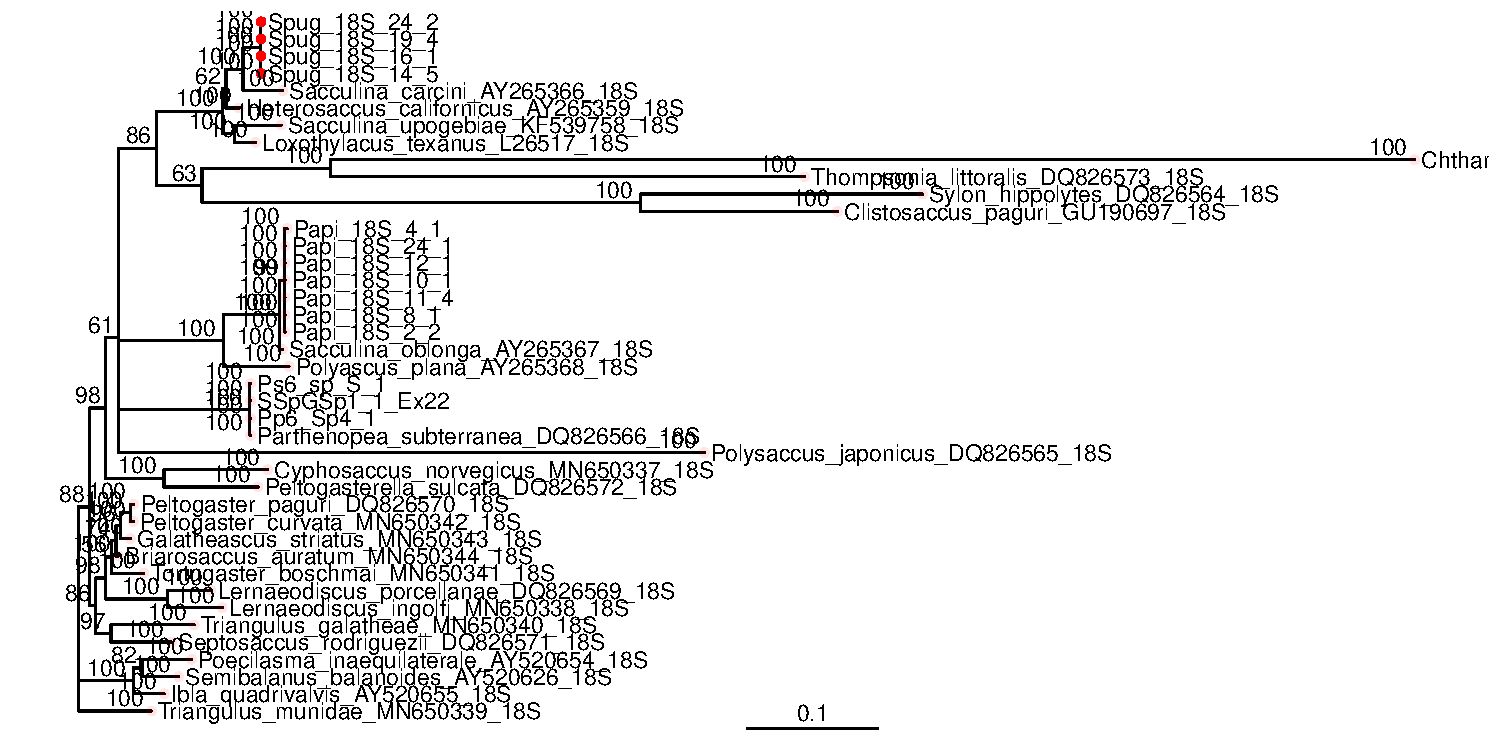
\includegraphics[keepaspectratio]{13_Phylogeny_files/figure-beamer/unnamed-chunk-14-1.pdf}}
\end{frame}

\begin{frame}[fragile]{Визуализация нескольких необходимых участков
дерева}
\protect\phantomsection\label{ux432ux438ux437ux443ux430ux43bux438ux437ux430ux446ux438ux44f-ux43dux435ux441ux43aux43eux43bux44cux43aux438ux445-ux43dux435ux43eux431ux445ux43eux434ux438ux43cux44bux445-ux443ux447ux430ux441ux442ux43aux43eux432-ux434ux435ux440ux435ux432ux430}
\begin{Shaded}
\begin{Highlighting}[]
\DocumentationTok{\#\# добавляем парасаккулину}
\NormalTok{sac\_para\_nodes }\OtherTok{\textless{}{-}} \FunctionTok{list}\NormalTok{(}\StringTok{"Sacculina pugettiae"} \OtherTok{=} \FunctionTok{c}\NormalTok{(}\StringTok{"Spug\_18S\_14\_5"}\NormalTok{,}
                                                 \StringTok{"Spug\_18S\_16\_1"}\NormalTok{,}
                                                 \StringTok{"Spug\_18S\_19\_4"}\NormalTok{,}
                                                 \StringTok{"Spug\_18S\_24\_2"}\NormalTok{),}
                       \StringTok{"Parasacculina pilosella"} \OtherTok{=}\NormalTok{ nex\_rhiz}\SpecialCharTok{@}\NormalTok{phylo}\SpecialCharTok{$}\NormalTok{tip.label[}\DecValTok{18}\SpecialCharTok{:}\DecValTok{24}\NormalTok{])}

\NormalTok{sac\_para\_otus }\OtherTok{\textless{}{-}} \FunctionTok{groupOTU}\NormalTok{(nex\_rhiz, sac\_para\_nodes)}
\end{Highlighting}
\end{Shaded}
\end{frame}

\begin{frame}[fragile]{Визуализация}
\protect\phantomsection\label{ux432ux438ux437ux443ux430ux43bux438ux437ux430ux446ux438ux44f}
\begin{Shaded}
\begin{Highlighting}[]
\NormalTok{(gg\_spug\_ppil }\OtherTok{\textless{}{-}}  \FunctionTok{ggtree}\NormalTok{(sac\_para\_otus) }\SpecialCharTok{+}
  \FunctionTok{geom\_tiplab}\NormalTok{(}\AttributeTok{size =} \DecValTok{4}\NormalTok{) }\SpecialCharTok{+}
  \FunctionTok{geom\_nodelab}\NormalTok{() }\SpecialCharTok{+}
  \FunctionTok{geom\_treescale}\NormalTok{() }\SpecialCharTok{+}
  \FunctionTok{geom\_tippoint}\NormalTok{(}\FunctionTok{aes}\NormalTok{(}\AttributeTok{col =}\NormalTok{ group)) }\SpecialCharTok{+}
  \FunctionTok{scale\_color\_manual}\NormalTok{(}\AttributeTok{values=}\FunctionTok{c}\NormalTok{(}\StringTok{"black"}\NormalTok{, }\StringTok{"blue"}\NormalTok{, }\StringTok{"orange"}\NormalTok{)) }\SpecialCharTok{+}
  \FunctionTok{geom\_text}\NormalTok{(}\FunctionTok{aes}\NormalTok{(}\AttributeTok{label =}\NormalTok{ prob\_percent),}
            \AttributeTok{hjust =} \FloatTok{1.2}\NormalTok{, }\AttributeTok{vjust =} \SpecialCharTok{{-}}\FloatTok{0.3}\NormalTok{))}
\end{Highlighting}
\end{Shaded}

\pandocbounded{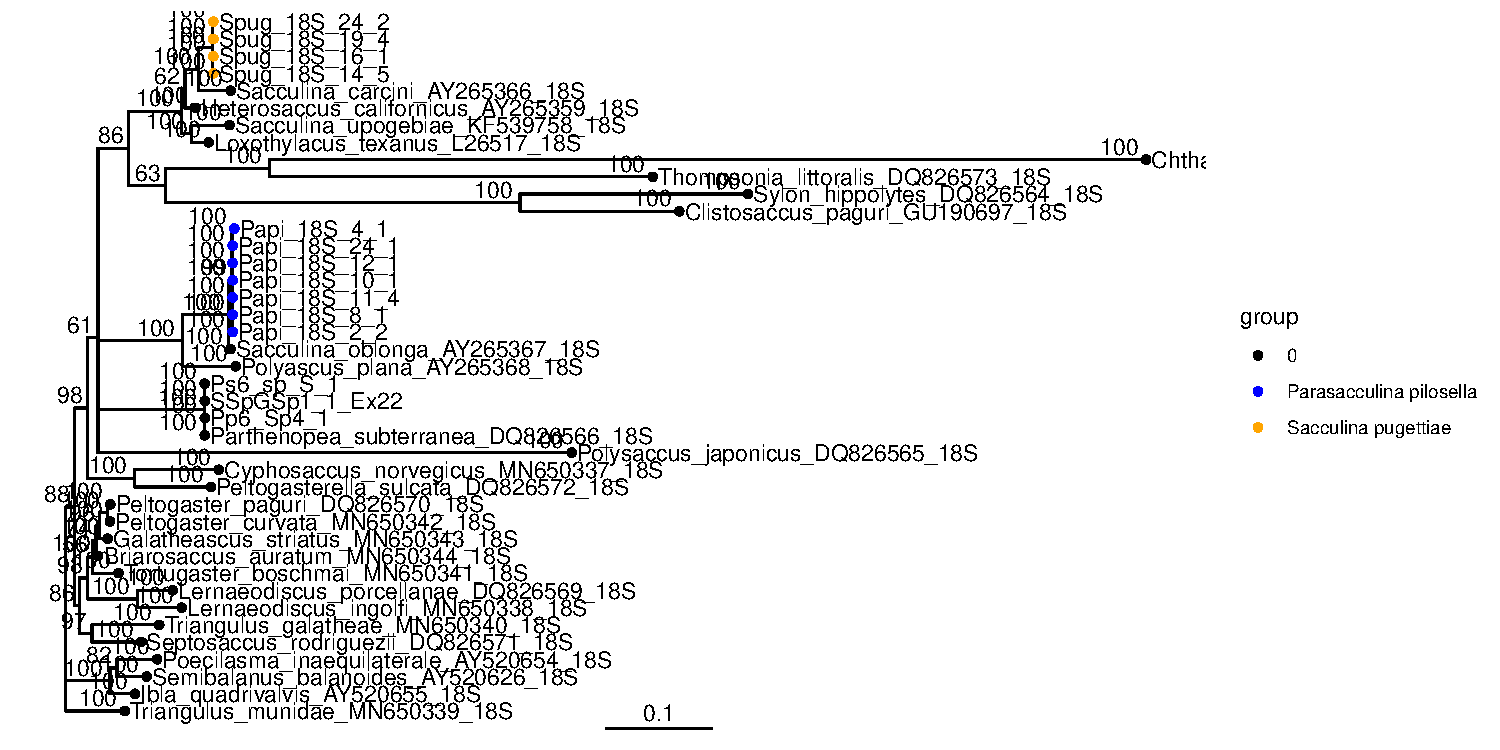
\includegraphics[keepaspectratio]{13_Phylogeny_files/figure-beamer/unnamed-chunk-16-1.pdf}}
\end{frame}

\begin{frame}[fragile]{Выделение нужных узлов на дереве}
\protect\phantomsection\label{ux432ux44bux434ux435ux43bux435ux43dux438ux435-ux43dux443ux436ux43dux44bux445-ux443ux437ux43bux43eux432-ux43dux430-ux434ux435ux440ux435ux432ux435}
Подсматриваем нумерацию нужных узлов.

\begin{Shaded}
\begin{Highlighting}[]
\FunctionTok{ggtree}\NormalTok{(sac\_para\_otus) }\SpecialCharTok{+}
  \FunctionTok{geom\_tiplab}\NormalTok{(}\AttributeTok{size =} \DecValTok{4}\NormalTok{) }\SpecialCharTok{+}
  \FunctionTok{geom\_treescale}\NormalTok{() }\SpecialCharTok{+}
  \FunctionTok{geom\_text}\NormalTok{(}\FunctionTok{aes}\NormalTok{(}\AttributeTok{label=}\NormalTok{node), }\AttributeTok{hjust=}\FloatTok{1.2}\NormalTok{, }\AttributeTok{vjust =} \SpecialCharTok{{-}}\NormalTok{.}\DecValTok{3}\NormalTok{)}
\end{Highlighting}
\end{Shaded}

\pandocbounded{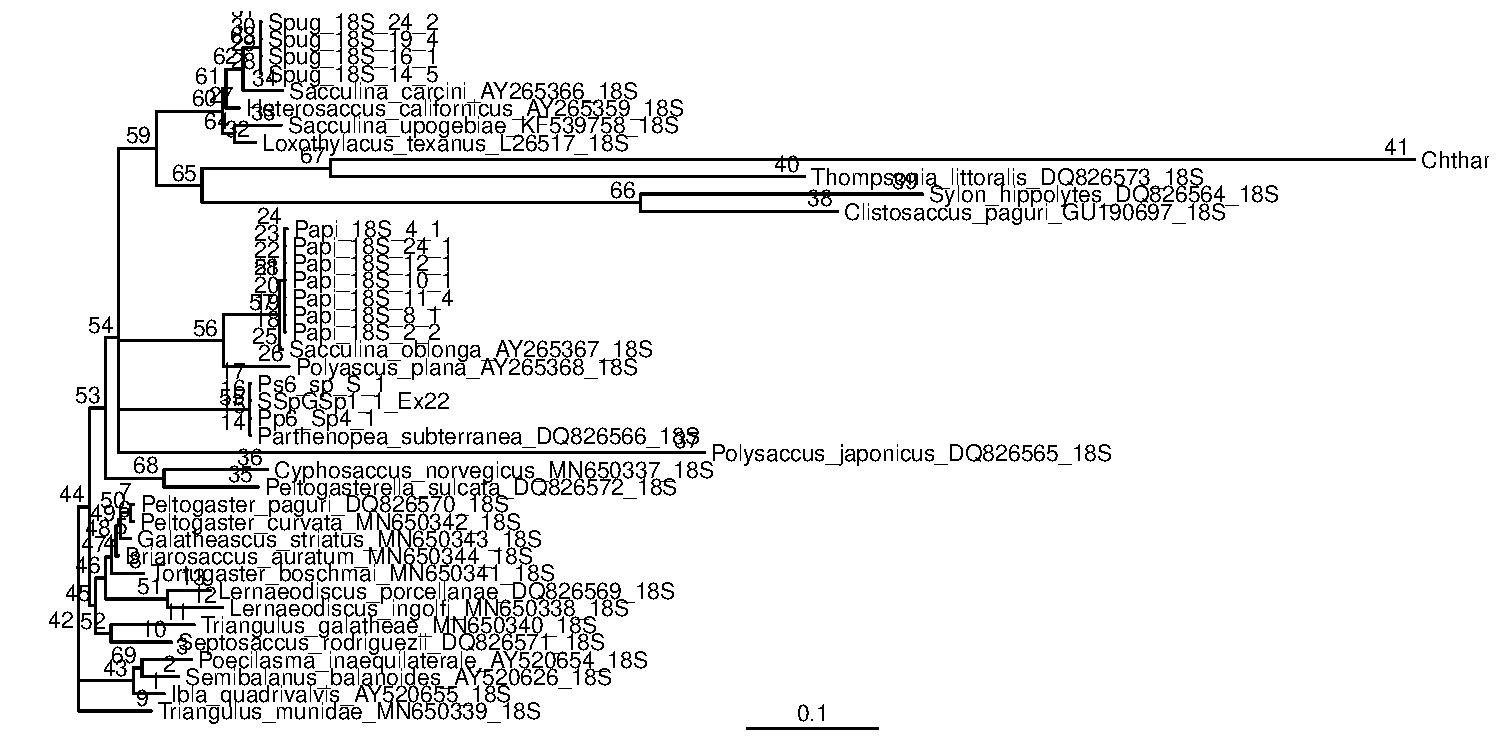
\includegraphics[keepaspectratio]{13_Phylogeny_files/figure-beamer/unnamed-chunk-17-1.pdf}}
\end{frame}

\begin{frame}[fragile]{Графическое изображение нужных узлов:
раскрашивание ветвей}
\protect\phantomsection\label{ux433ux440ux430ux444ux438ux447ux435ux441ux43aux43eux435-ux438ux437ux43eux431ux440ux430ux436ux435ux43dux438ux435-ux43dux443ux436ux43dux44bux445-ux443ux437ux43bux43eux432-ux440ux430ux441ux43aux440ux430ux448ux438ux432ux430ux43dux438ux435-ux432ux435ux442ux432ux435ux439}
\begin{Shaded}
\begin{Highlighting}[]
\FunctionTok{ggtree}\NormalTok{(sac\_para\_otus) }\SpecialCharTok{+}
  \FunctionTok{geom\_tiplab}\NormalTok{(}\AttributeTok{size =} \DecValTok{4}\NormalTok{) }\SpecialCharTok{+} \FunctionTok{geom\_nodelab}\NormalTok{() }\SpecialCharTok{+} \FunctionTok{geom\_treescale}\NormalTok{() }\SpecialCharTok{+}
  \FunctionTok{geom\_hilight}\NormalTok{(}\AttributeTok{node =} \DecValTok{63}\NormalTok{, }\AttributeTok{fill =} \StringTok{"orange"}\NormalTok{) }\SpecialCharTok{+}
  \FunctionTok{geom\_hilight}\NormalTok{(}\AttributeTok{node =} \DecValTok{58}\NormalTok{, }\AttributeTok{fill =} \StringTok{"blue"}\NormalTok{) }\SpecialCharTok{+}
  \FunctionTok{geom\_text}\NormalTok{(}\FunctionTok{aes}\NormalTok{(}\AttributeTok{label =}\NormalTok{ prob\_percent),}
          \AttributeTok{hjust =} \FloatTok{1.2}\NormalTok{, }\AttributeTok{vjust =} \SpecialCharTok{{-}}\FloatTok{0.3}\NormalTok{)}
\end{Highlighting}
\end{Shaded}

\pandocbounded{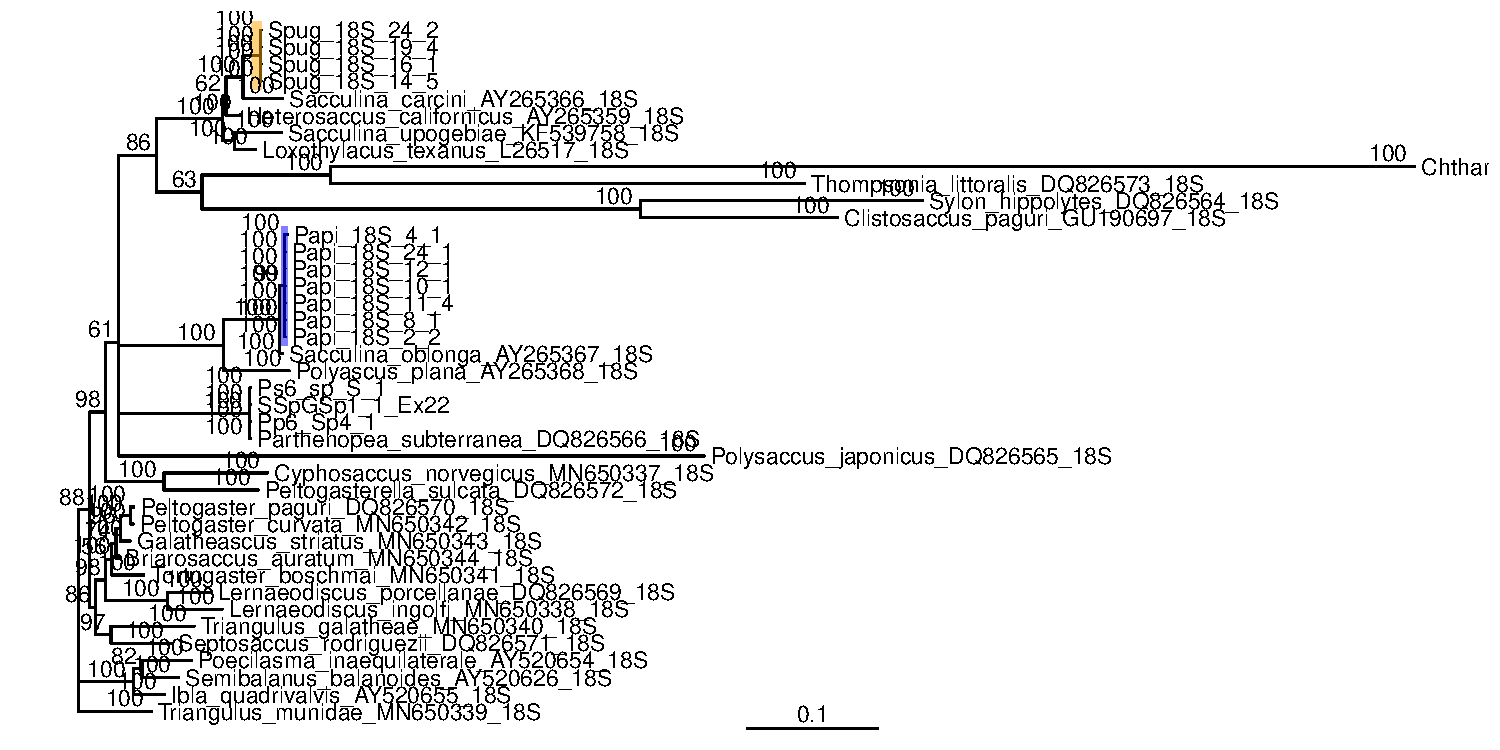
\includegraphics[keepaspectratio]{13_Phylogeny_files/figure-beamer/unnamed-chunk-18-1.pdf}}
\end{frame}

\begin{frame}[fragile]{Графическое изображение нужных узлов:
раскрашивание ветвей: выделение узлов}
\protect\phantomsection\label{ux433ux440ux430ux444ux438ux447ux435ux441ux43aux43eux435-ux438ux437ux43eux431ux440ux430ux436ux435ux43dux438ux435-ux43dux443ux436ux43dux44bux445-ux443ux437ux43bux43eux432-ux440ux430ux441ux43aux440ux430ux448ux438ux432ux430ux43dux438ux435-ux432ux435ux442ux432ux435ux439-ux432ux44bux434ux435ux43bux435ux43dux438ux435-ux443ux437ux43bux43eux432}
\begin{Shaded}
\begin{Highlighting}[]
\FunctionTok{ggtree}\NormalTok{(sac\_para\_otus) }\SpecialCharTok{+} \FunctionTok{geom\_tiplab}\NormalTok{(}\AttributeTok{size =} \DecValTok{4}\NormalTok{) }\SpecialCharTok{+}
  \FunctionTok{geom\_text}\NormalTok{(}\FunctionTok{aes}\NormalTok{(}\AttributeTok{label =}\NormalTok{ prob\_percent), }\AttributeTok{hjust =} \FloatTok{1.2}\NormalTok{, }\AttributeTok{vjust =} \SpecialCharTok{{-}}\FloatTok{0.3}\NormalTok{) }\SpecialCharTok{+}
  \FunctionTok{geom\_cladelabel}\NormalTok{(}\AttributeTok{node =} \DecValTok{63}\NormalTok{, }\AttributeTok{label=}\StringTok{"Sacculina pugettiae"}\NormalTok{,}
                \AttributeTok{color =} \StringTok{\textquotesingle{}orange\textquotesingle{}}\NormalTok{, }\AttributeTok{offset =} \FloatTok{0.3}\NormalTok{, }\AttributeTok{hjust =} \SpecialCharTok{{-}}\FloatTok{0.1}\NormalTok{) }\SpecialCharTok{+}
  \FunctionTok{geom\_cladelabel}\NormalTok{(}\AttributeTok{node =} \DecValTok{58}\NormalTok{, }\AttributeTok{label=}\StringTok{"Parasacculina pilosella"}\NormalTok{,}
                \AttributeTok{color =} \StringTok{\textquotesingle{}blue\textquotesingle{}}\NormalTok{, }\AttributeTok{offset =} \FloatTok{0.28}\NormalTok{, }\AttributeTok{hjust =} \SpecialCharTok{{-}}\FloatTok{0.1}\NormalTok{)}
\end{Highlighting}
\end{Shaded}

\pandocbounded{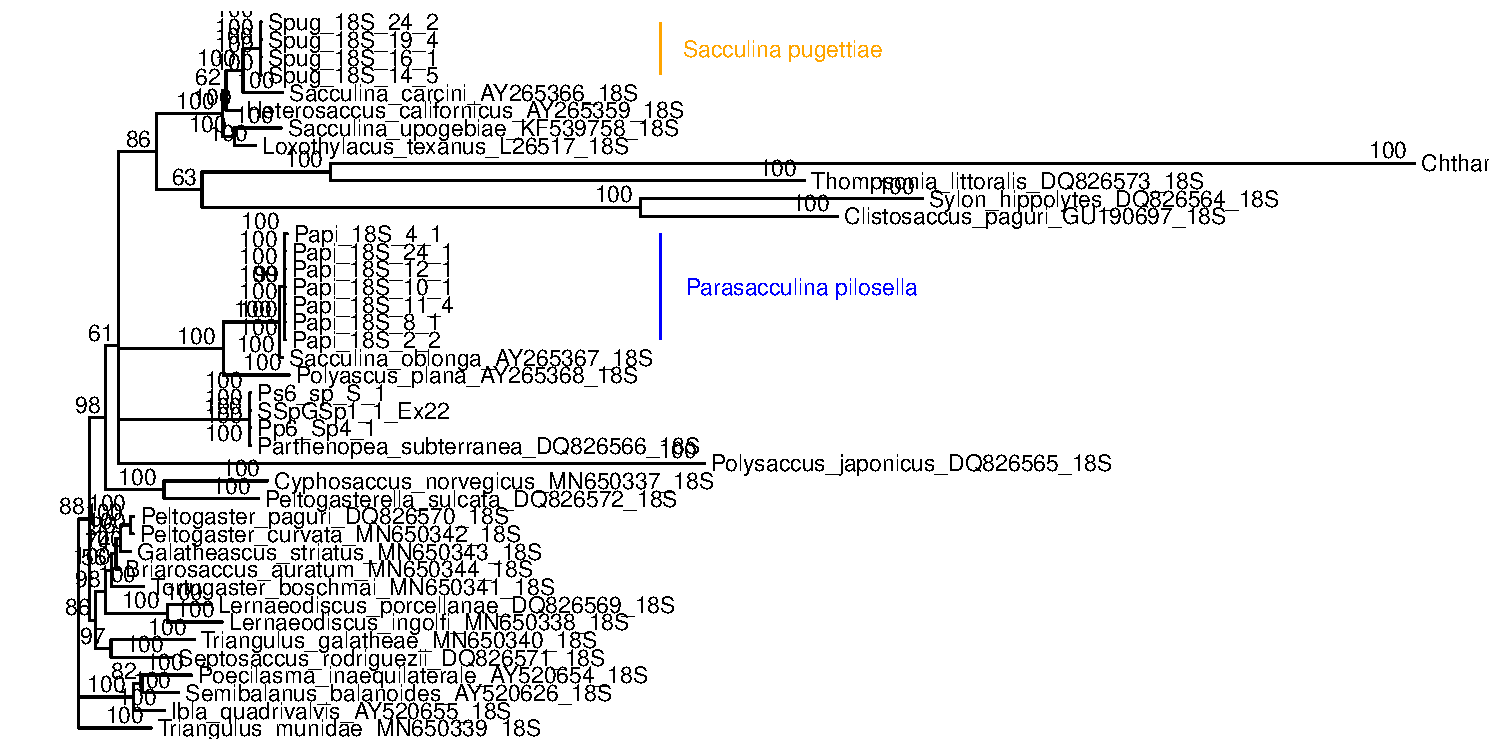
\includegraphics[keepaspectratio]{13_Phylogeny_files/figure-beamer/unnamed-chunk-19-1.pdf}}
\end{frame}

\begin{frame}[fragile]{Сравнение разных деревьев}
\protect\phantomsection\label{ux441ux440ux430ux432ux43dux435ux43dux438ux435-ux440ux430ux437ux43dux44bux445-ux434ux435ux440ux435ux432ux44cux435ux432}
Возьмём дерево, полученное методом максимального правдоподобие и с
использованием заведомо неправильной модели (JC69).

\begin{Shaded}
\begin{Highlighting}[]
\NormalTok{jc69 }\OtherTok{\textless{}{-}} \FunctionTok{read.tree}\NormalTok{(}\StringTok{"data/18S\_JC69\_sac\_parasac.treefile"}\NormalTok{)}

\FunctionTok{ggtree}\NormalTok{(jc69) }\SpecialCharTok{+}
  \FunctionTok{geom\_tiplab}\NormalTok{(}\AttributeTok{size =} \DecValTok{4}\NormalTok{) }\SpecialCharTok{+} \FunctionTok{geom\_treescale}\NormalTok{() }\SpecialCharTok{+}
  \FunctionTok{geom\_text}\NormalTok{(}\FunctionTok{aes}\NormalTok{(}\AttributeTok{label=}\NormalTok{node), }\AttributeTok{hjust=}\FloatTok{1.2}\NormalTok{, }\AttributeTok{vjust =} \SpecialCharTok{{-}}\NormalTok{.}\DecValTok{3}\NormalTok{)}
\end{Highlighting}
\end{Shaded}

\pandocbounded{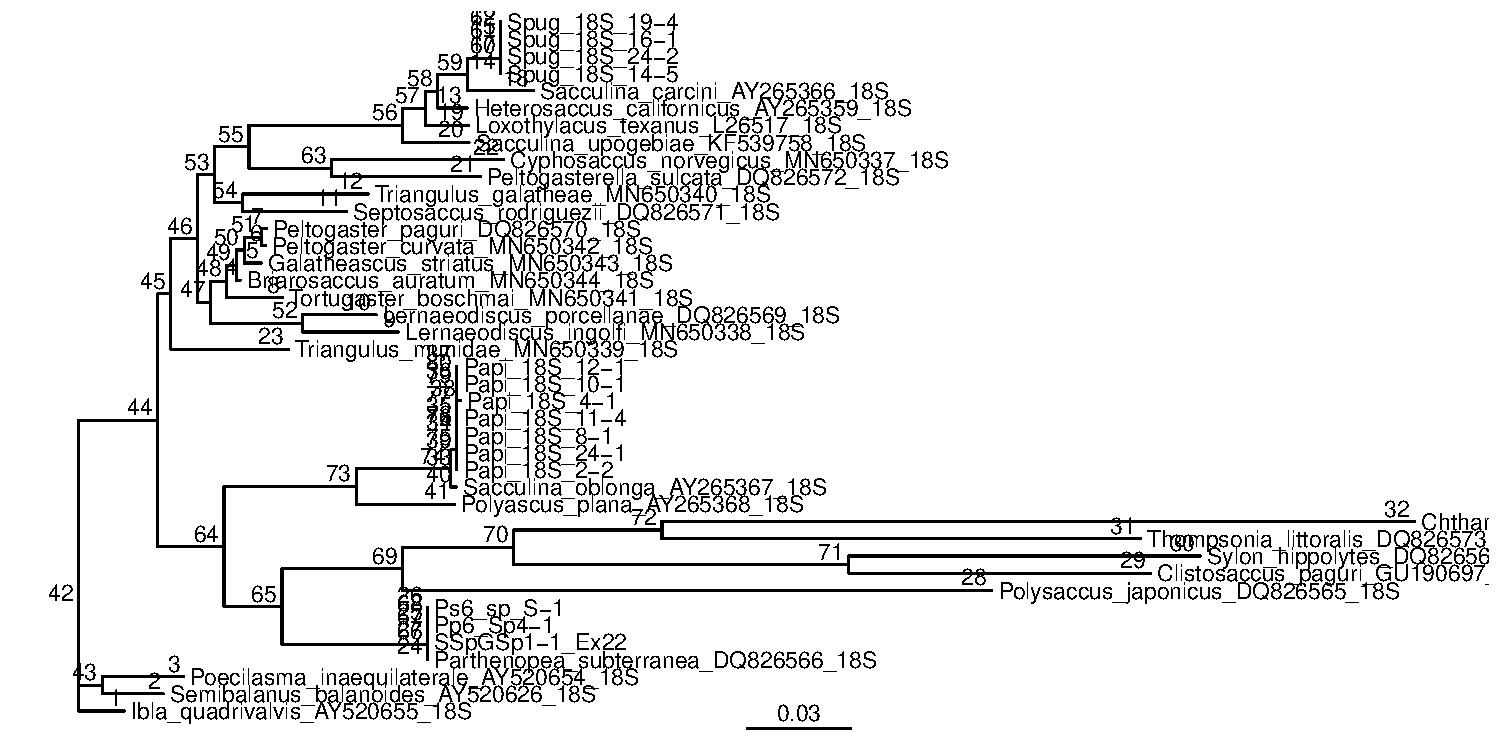
\includegraphics[keepaspectratio]{13_Phylogeny_files/figure-beamer/unnamed-chunk-20-1.pdf}}
\end{frame}

\begin{frame}[fragile]{Укоренение дерева, построенного по другой модели
замен}
\protect\phantomsection\label{ux443ux43aux43eux440ux435ux43dux435ux43dux438ux435-ux434ux435ux440ux435ux432ux430-ux43fux43eux441ux442ux440ux43eux435ux43dux43dux43eux433ux43e-ux43fux43e-ux434ux440ux443ux433ux43eux439-ux43cux43eux434ux435ux43bux438-ux437ux430ux43cux435ux43d}
\begin{Shaded}
\begin{Highlighting}[]
\NormalTok{jc69 }\OtherTok{\textless{}{-}} \FunctionTok{root}\NormalTok{(jc69, }\AttributeTok{node =} \DecValTok{42}\NormalTok{)}

\NormalTok{(jc69\_tree }\OtherTok{\textless{}{-}} \FunctionTok{ggtree}\NormalTok{(jc69) }\SpecialCharTok{+} \FunctionTok{geom\_tiplab}\NormalTok{(}\AttributeTok{size =} \DecValTok{4}\NormalTok{) }\SpecialCharTok{+}
  \FunctionTok{geom\_nodelab}\NormalTok{(}\AttributeTok{hjust =} \FloatTok{1.2}\NormalTok{, }\AttributeTok{vjust =} \SpecialCharTok{{-}}\FloatTok{0.3}\NormalTok{) }\SpecialCharTok{+} \FunctionTok{geom\_treescale}\NormalTok{())}
\end{Highlighting}
\end{Shaded}

\pandocbounded{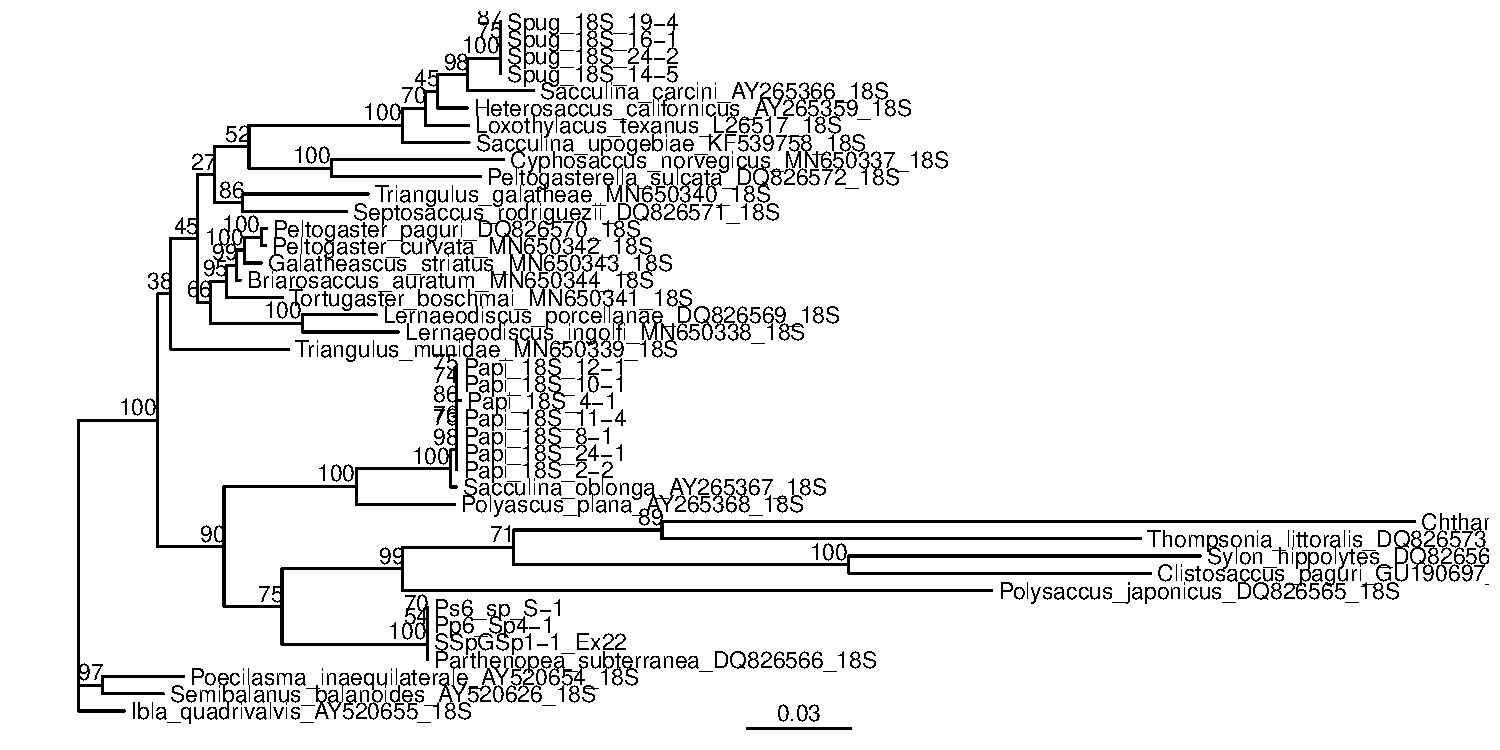
\includegraphics[keepaspectratio]{13_Phylogeny_files/figure-beamer/unnamed-chunk-21-1.pdf}}
\end{frame}

\begin{frame}[fragile]{Построение кофилогении}
\protect\phantomsection\label{ux43fux43eux441ux442ux440ux43eux435ux43dux438ux435-ux43aux43eux444ux438ux43bux43eux433ux435ux43dux438ux438}
Отображение двух графиков, построенных посредством \texttt{ggtree}
вместе.

\begin{Shaded}
\begin{Highlighting}[]
\FunctionTok{library}\NormalTok{(ggpubr)}
\FunctionTok{ggarrange}\NormalTok{(gtr\_tree, jc69\_tree)}
\end{Highlighting}
\end{Shaded}

\pandocbounded{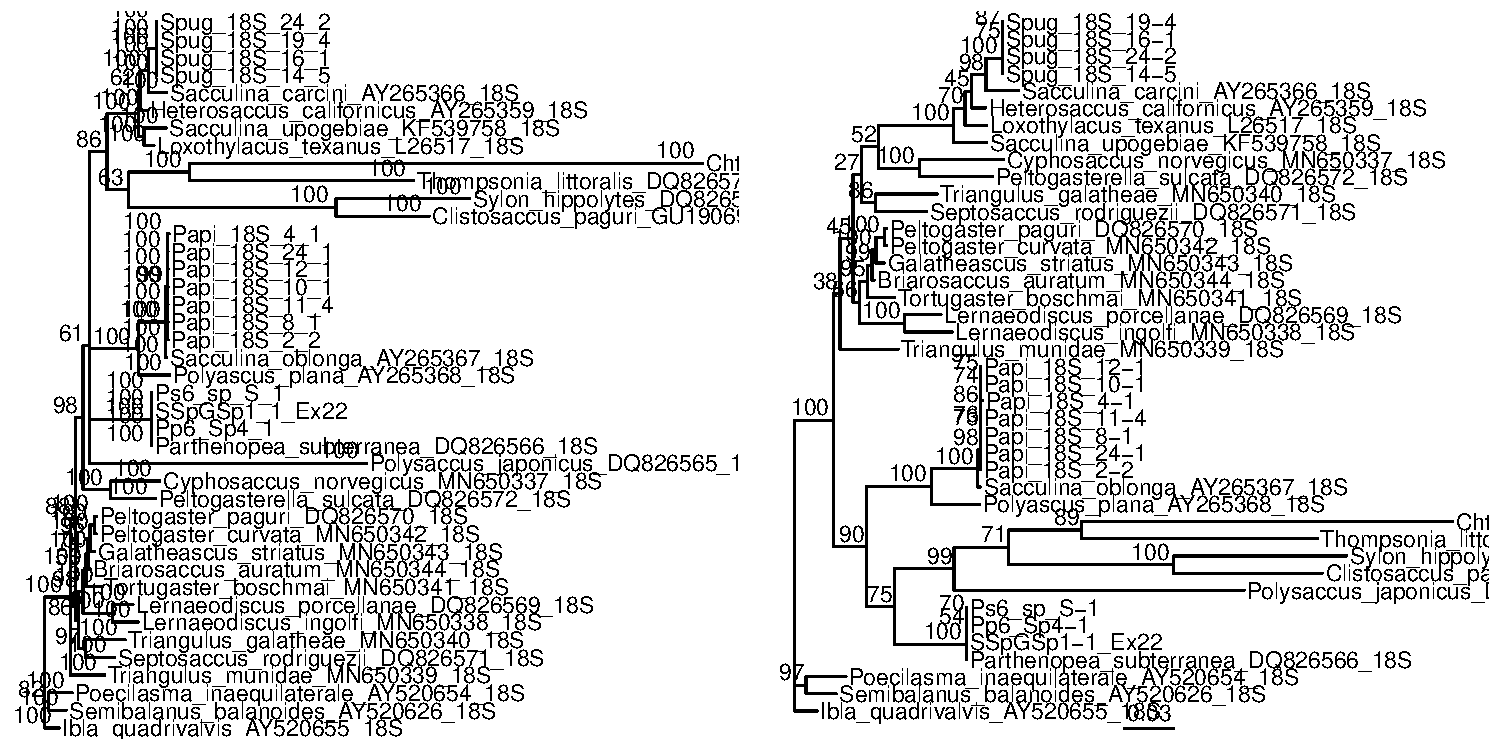
\includegraphics[keepaspectratio]{13_Phylogeny_files/figure-beamer/unnamed-chunk-22-1.pdf}}
\end{frame}

\begin{frame}[fragile]{Дерево, построенное с помощью пакета ape}
\protect\phantomsection\label{ux434ux435ux440ux435ux432ux43e-ux43fux43eux441ux442ux440ux43eux435ux43dux43dux43eux435-ux441-ux43fux43eux43cux43eux449ux44cux44e-ux43fux430ux43aux435ux442ux430-ape}
\begin{Shaded}
\begin{Highlighting}[]
\FunctionTok{library}\NormalTok{(ape)}
\FunctionTok{cophyloplot}\NormalTok{(nex\_rhiz}\SpecialCharTok{@}\NormalTok{phylo, jc69, }\AttributeTok{length.line=}\DecValTok{4}\NormalTok{, }\AttributeTok{space=}\DecValTok{40}\NormalTok{)}
\end{Highlighting}
\end{Shaded}

\begin{verbatim}
[1] "No association matrix specified. Links will be omitted."
\end{verbatim}

\pandocbounded{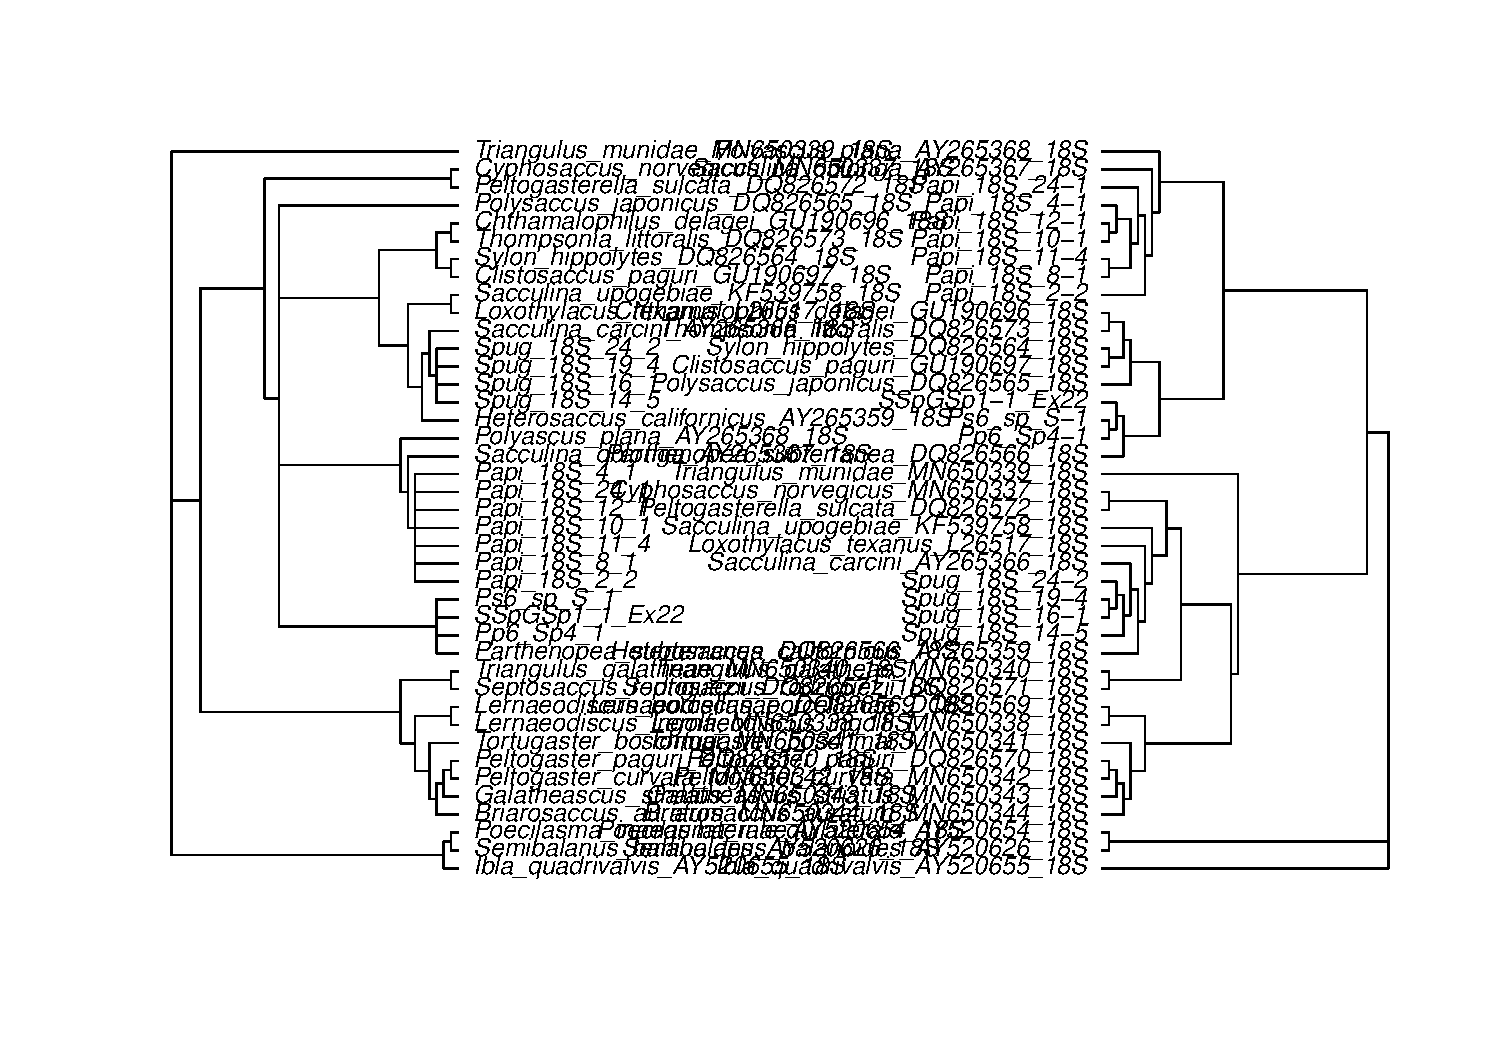
\includegraphics[keepaspectratio]{13_Phylogeny_files/figure-beamer/unnamed-chunk-23-1.pdf}}
\end{frame}

\begin{frame}[fragile]{Дерево, построенное с помощью пакета phytools}
\protect\phantomsection\label{ux434ux435ux440ux435ux432ux43e-ux43fux43eux441ux442ux440ux43eux435ux43dux43dux43eux435-ux441-ux43fux43eux43cux43eux449ux44cux44e-ux43fux430ux43aux435ux442ux430-phytools}
\begin{Shaded}
\begin{Highlighting}[]
\FunctionTok{library}\NormalTok{(phytools)}
\NormalTok{trees.cophylo}\OtherTok{\textless{}{-}}\FunctionTok{cophylo}\NormalTok{(nex\_rhiz}\SpecialCharTok{@}\NormalTok{phylo, jc69, }\AttributeTok{rotate =} \ConstantTok{TRUE}\NormalTok{)}
\end{Highlighting}
\end{Shaded}

\begin{verbatim}
Rotating nodes to optimize matching...
Done.
\end{verbatim}

\begin{Shaded}
\begin{Highlighting}[]
\FunctionTok{png}\NormalTok{(}\StringTok{"cophyplot.png"}\NormalTok{, }\AttributeTok{width =} \DecValTok{1200}\NormalTok{, }\AttributeTok{height =} \DecValTok{800}\NormalTok{)}
\FunctionTok{plot}\NormalTok{(trees.cophylo, }\AttributeTok{link.type =} \StringTok{"curved"}\NormalTok{, }\AttributeTok{link.lwd =} \DecValTok{4}\NormalTok{,}
     \AttributeTok{link.lty=}\StringTok{"solid"}\NormalTok{, }\AttributeTok{link.col =} \StringTok{"blue"}\NormalTok{, }\AttributeTok{size =} \DecValTok{1}\NormalTok{)}
\FunctionTok{dev.off}\NormalTok{()}
\end{Highlighting}
\end{Shaded}

\begin{verbatim}
pdf 
  2 
\end{verbatim}
\end{frame}

\begin{frame}{Дерево, построенное с помощью пакета phytools}
\protect\phantomsection\label{ux434ux435ux440ux435ux432ux43e-ux43fux43eux441ux442ux440ux43eux435ux43dux43dux43eux435-ux441-ux43fux43eux43cux43eux449ux44cux44e-ux43fux430ux43aux435ux442ux430-phytools-1}
\pandocbounded{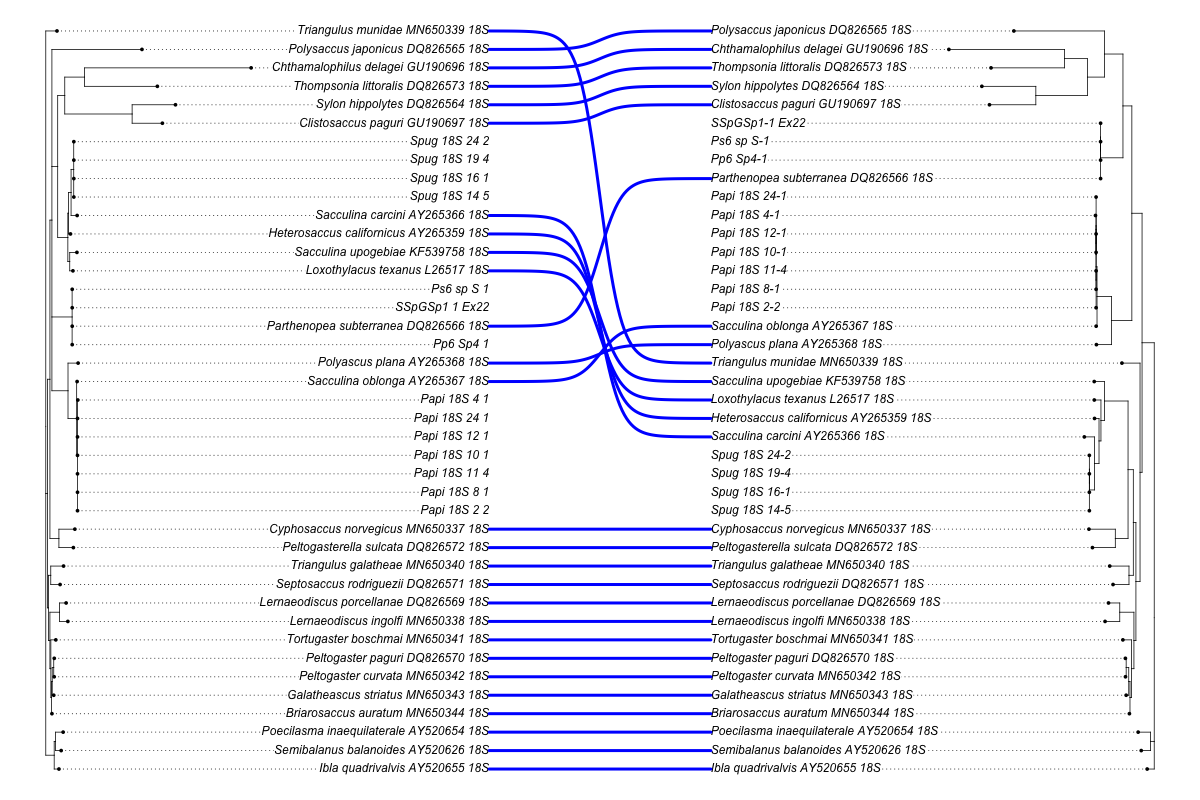
\includegraphics[keepaspectratio]{cophyplot.png}}
\end{frame}

\begin{frame}{Дополнительные ресурсы}
\protect\phantomsection\label{ux434ux43eux43fux43eux43bux43dux438ux442ux435ux43bux44cux43dux44bux435-ux440ux435ux441ux443ux440ux441ux44b}
\begin{itemize}
\item
  Lemey, P., Salemi, M., \& Vandamme, A. M. (Eds.). (2009). The
  phylogenetic handbook: a practical approach to phylogenetic analysis
  and hypothesis testing. Cambridge University Press.
\item
  Paradis, E. (2012). Analysis of Phylogenetics and Evolution with R
  (Vol. 2). New York: Springer.
\item
  Курс ``Молекулярная филогенетика'' на Stepik от
  \href{https://stepik.org/course/2054/syllabus}{Института
  Биоинформатики в лице Полины Дроздовой}
\end{itemize}
\end{frame}




\end{document}
